\chapter{Inverse Synthesis Experiment}
\label{chapter:inverse_synth_experiment}

This chapter presents an inverse synthesis experiment that was conducted to compare some of the recent approaches that have been used in previous work. The methodology used for this experiment was modelled after Yee-King et al.'s study on deep learning for automatic synthesizer programming \cite{yee2018automatic}, but with a simplified synthesizer configuration and a unique set of estimators. In total ten different methods for inverse synthesis were compared, including eight deep learning models based on previous work \cite{barkan2019inversynth, yee2018automatic} and two versions of a genetic algorithm \cite{horner1993machine, tatar2016automatic}. A VST software emulation of the Yamaha DX7 FM synthesizer called \textit{Dexed} was used with a restricted subset of the parameters. While Dexed has been used in previous work for inverse synthesis \cite{yee2018automatic, luke2019stochastic, le2021improving, masudo2021quality}, each work has used a unique subset of parameters and sounds for their experiments. Depending on the parameters that are selected, the difficulty of the problem varies considerably. In this experiment we propose a minimal subset of nine parameters to reduce the complexity of the problem and to provide a benchmark for evaluation.

The following section describes in more detail the methods used for this experiment including the precise configuration of the synthesizer, the dataset used for training, and the various techniques compared. Section \ref{sec:inverse-synth-eval} describes the methods used for evaluation and the results of this evaluation. Section \ref{sec:inverse-synth-discuss} presents a discussion of the results and some of the challenges associated with the inverse synthesis problem. In alignment with Vandewalle et al.'s criteria for reproducible research, implementation details, code, and datasets are all available on the \mintinline{python}{spiegelib} online documentation.\footnote{\url{https://spiegelib.github.io/spiegelib/examples/fm_sound_match.html}}

\section{Synthesizer Configuration}
The first step in the experiment was defining the synthesizer setup. The $Dexed$ VST instrument was selected for this experiment for a number of reasons: 1) it is an FM synthesizer that is modelled closely after the Yamaha DX7 synthesizer which is both widely used as well as notoriously difficult to program, 2) Dexed is open-source and free to use which makes it easy for the results to be reproduced, and 3) it has been used in a number of previous works on inverse synthesis \cite{yee2018automatic, luke2019stochastic, le2021improving, masudo2021quality}. An image of the $Dexed$ interface is shown in figure \ref{fig:dexed}. Dexed has 155 automatable parameters that are accessible for control from a DAW, which represent the parameters that are available for programming via inverse synthesis. A subset of nine of these parameters were used in this experiment to turn $Dexed$ into a simple two-operator FM synthesizer. In this configuration the second operator modulates the frequency of the first operator. A block diagram showing the resulting synth configuration is shown in figure \ref{fig:two_op_fm_block}. The subset of nine parameters control the amplitude envelope and tuning of the modulating oscillator; this simple synthesizer can produce a wide range of timbres that evolve in various ways over time based on the amplitude envelope of the modulating oscillator. An overview of these nine parameters is given in table \ref{tbl:dexed-params}.

\begin{figure}[ht]
    \centering
    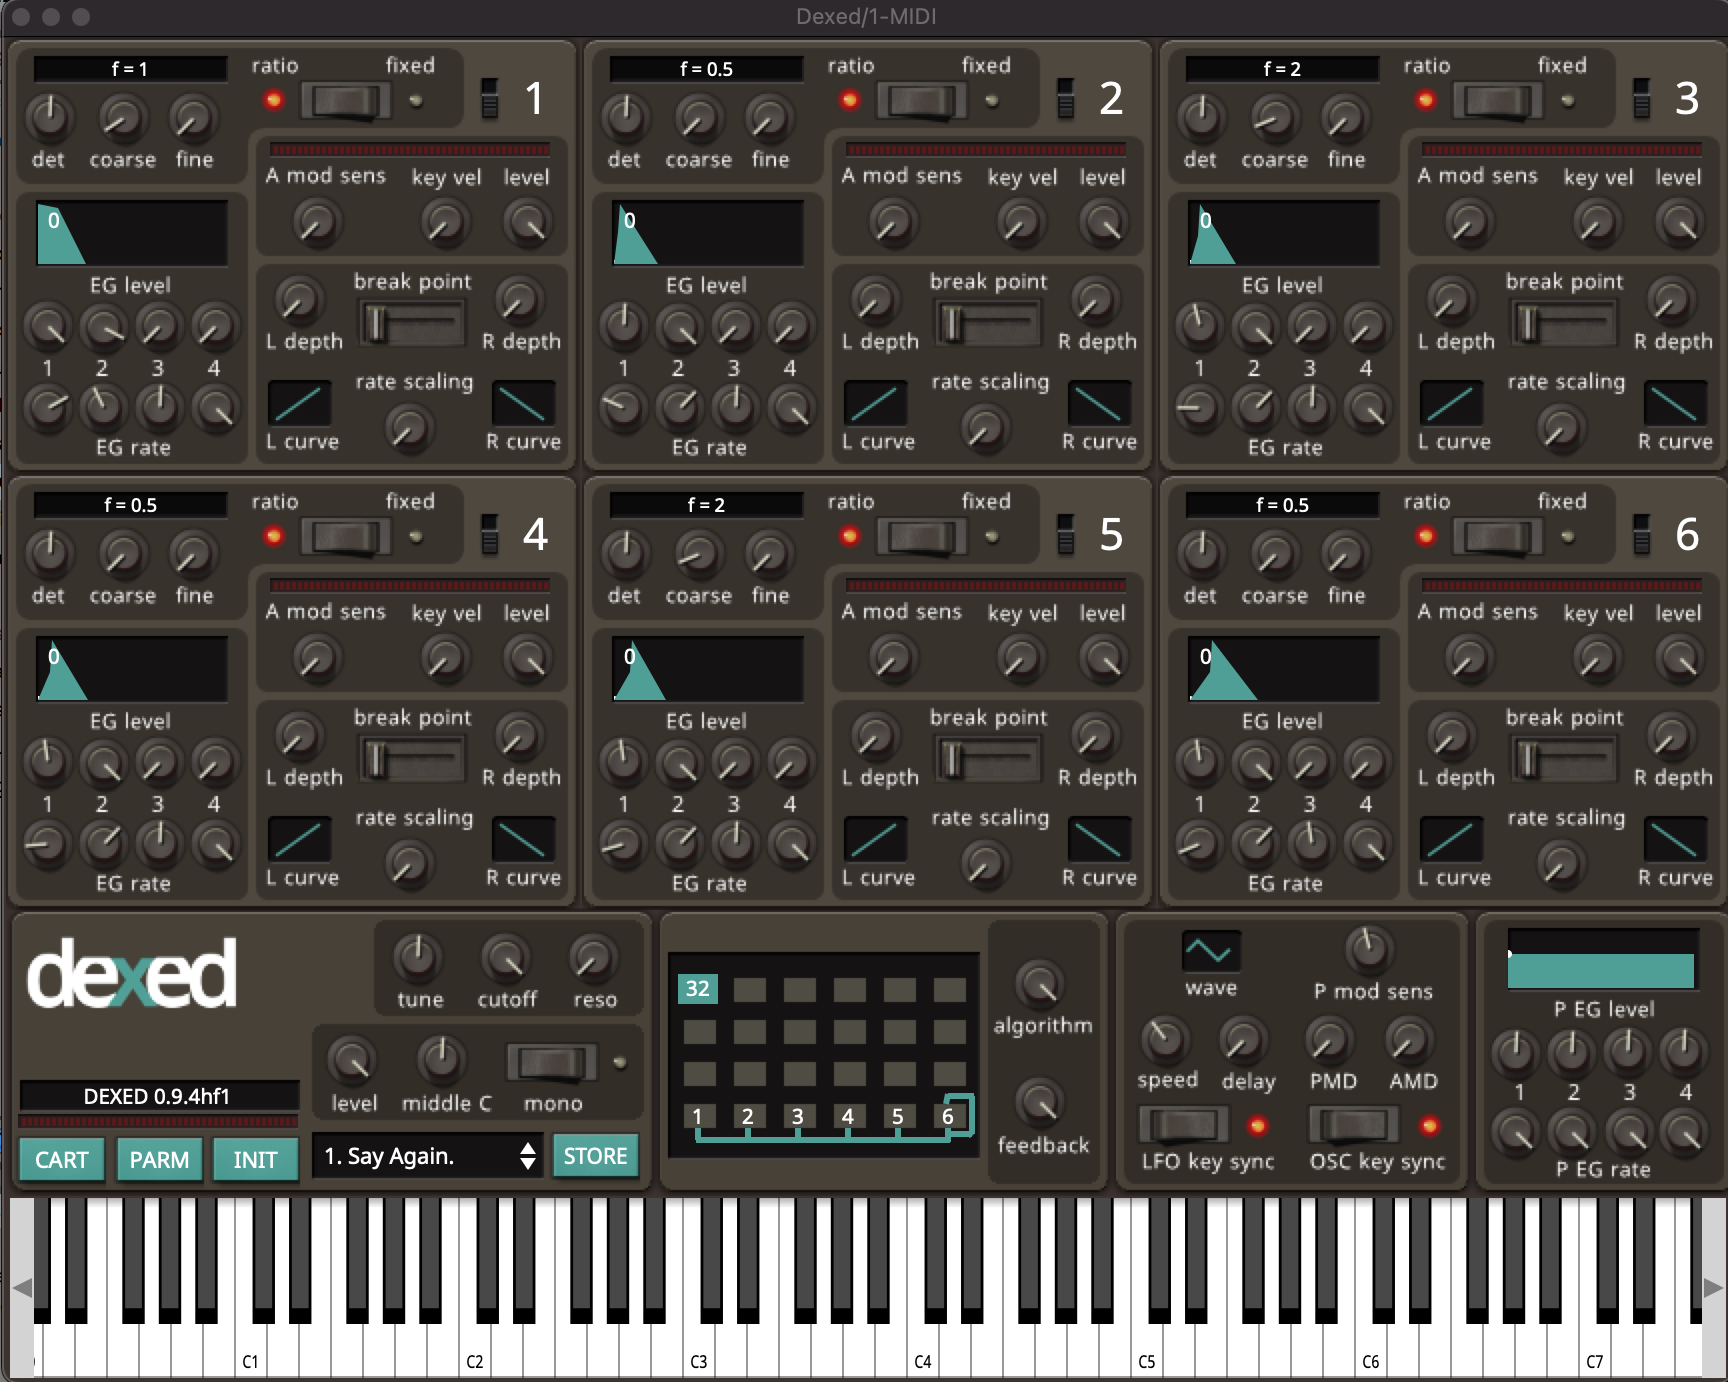
\includegraphics[width=0.6\textwidth]{figures/spiegelib/dexed.png}
    \caption{The Dexed synthesizer interface. Dexed is an open-source emulation of the Yamaha DX7 FM synthesizer and it was used in the experiments in this chapter/}
    \label{fig:dexed}
\end{figure}

\begin{figure}[ht]
    \centering
    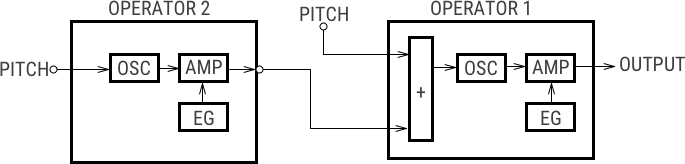
\includegraphics[width=0.9\textwidth]{figures/spiegelib/two_op_fm_block.png}
    \caption{Block diagram of a two operator FM synthesizer. Dexed has six independent operators that can be configured in various ways, however for the experiments conducted here only the first two operators were used and were setup in this configuration.}
    \label{fig:two_op_fm_block}
\end{figure}

\begin{table}[ht]
\centering
\caption{Synthesis parameters used in experiment}
\label{tbl:dexed-params}
%\def\arraystretch{1.5}%  1 is the default, change whatever you need
\begin{tabular}{l|l}
\toprule
Parameter     & Description                                                                                  \\
\midrule
OP2 EG RATE 2 & \multirow{3}{*}{\parbox{0.70\linewidth}{Controls the duration of stages 2-4 of the envelope generator applied the the amplitude of operator 2}} \\
OP2 EG RATE 3 \\
OP2 EG RATE 4 \\
\midrule
OP2 EG LEVEL 2 & \multirow{3}{*}{\parbox{0.6\linewidth}{Controls level of the envelope generator at stages 2-4, which is applied the amplitude of operator 2}} \\
OP2 EG LEVEL 3 \\
OP2 EG LEVEL 4 \\
\midrule
OP2 F COARSE & \multirow{2}{*}{\parbox{0.6\linewidth}{Frequency of second operator in relation to the fundamental frequency of the MIDI pitch. Coarse tuning is an integer ratio from $\frac{1}{2}$ to 31. Fine tuning allows for smaller non-integer adjustments.}} \\[2.75ex]
OP2 F FINE \\[2.75ex]
\midrule
OP2 OSC DETUNE & \multirow{1}{*}{\parbox{0.6\linewidth}{Detunes the second operator by $\pm$ 7 cents}}\\
\bottomrule                                                                                        
\end{tabular}
\end{table}
\vspace{1cm}

Each operator in $Dexed$ has a complex envelope generator (EG) that is used modulate the amplitude of that operator. The complex envelope generator has five independent stages that are controlled by a set of parameters that are used to adjust the length and amplitude of each stage. For this experiment, only the EG for the second operator had parameters for estimation: $LEVEL 2-4$ and $RATE 2-4$. The $RATE 1$ and $LEVEL 1$ parameters were locked to the minmimum rate and highest level, effectively turning off the initial rise portion of the envelope. Three parameters controlling the pitch and tuning of the second operator were also open for estimation. Although each of the included parameters control the amplitude EG and pitch of the operator in distinct ways, there is redundancy in the parameter spaced, i.e. different parameter settings could lead to the same auditory result. This redundancy represents one of the complexities of synthesizer parameter spaces and challenges in automatic synthesizer programming. This experiment intentionally seeks to explore the affect this redundancy has on each techniques ability to effectively match. All parameters have a normalized range from $[0-1]$ and mapping from this normalized range is handled internally by the Dexed code. The remainder of the available parameters in $Dexed$ are locked at values to create a simple sine wave generator that is being frequency modulated by the second operator. [ADD A TABLE IN APPENDIX FOR ALL THE PARAMETER VALUES]. The \mintinline{python}{SynthVST} class in spiegelib provides methods for overriding and freezing parameters as well as saving and loading parameter settings as JSON files. 

\begin{figure}[ht]
    \centering
    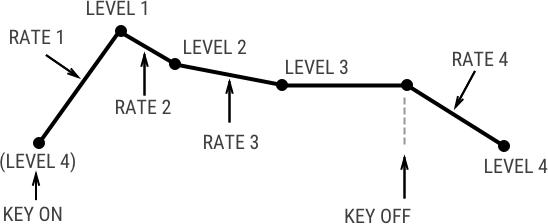
\includegraphics[width=0.75\textwidth]{figures/spiegelib/Yamaha DX7 Envelope.png}
    \caption{Diagram of an envelope generator in the Yamaha DX7 and Dexed. The envelope has five independent stages. During the first three stages the envelope moves linearly from level 4 to level 1, then to level 2, then to level 3. Each of these levels is controllable and the length of time taken to move to each level is also definable. This movement is triggered by a key-on event. Once the envelope has progressed to level 3 it stays at that level until a key-off event is received, at which point the envelope progresses back to level 4.}
    \label{fig:dx7_envelope}
\end{figure}


\section{Dataset Generation}
\label{sec:dataset-generation}

A dataset of synthesized audio paired with the parameters used for generation was required for training the deep learning models used in this experiment. Dataset creation consisted of sampling the parameter space, rendering the audio resulting from the parameters, and then transforming the audio into a suitable audio representation for each model. All audio was rendered by sending a single MIDI note to Dexed with a note value of 48 (C3 - $\approx 130.81$Hz) and length of one second. 60,000 examples were generated by uniformly sampling the nine parameters and rendering audio for one second; audio results were saved as wav files at a sampling rate of 44,100kHz. The parameter values were also saved alongside each example. This dataset was then split into a training and validation set with the training set containing 80\% of the samples. Once the audio dataset was created, audio representations were generated for each example.

\subsection{Audio Representations}
All the models received audio input that has been transformed into a more perceptually relevant representation. Two different representations were used. The fully-connected and recurrent models used a 13-band Mel-frequency cepstral coefficient (MFCC) representation, which was the same used by Yee-King \textit{et al.} \cite{yee2018automatic}, and the convolutional neural networks (CNNs) used a log-scaled Mel-spectrogram representation. Barkan \textit{et al.} \cite{barkan2019inversynth} used a STFT representation in their experiments with CNNs, however Mel-spectrograms provide a more perceptually relevant frequency scaling and has been used in recent work in audio representations \cite{cramer:learnmore:icassp:19, hershey2017cnn}.

The MFCCs were computed with 13-bands using a frame size of 2048 and a hop size of 1024, this resulted in 44 frames over the 1-second long input audio. To compute the Mel-spectrograms, a STFT was first computed using a frame-size of 2048 samples and a hop-size of 1024 samples. Each frame of the magnitude spectrogram was then converted to a power spectrum and then projected onto a 128 component Mel-frequency scale. The resulting Mel-spectrogram is then scaled to a log-scale, which is an amplitude scaling more reflective of human auditory perception of loudness. Equation \ref{ref:eq-log-scale} shows the calculation of the log-scaled Mel-spectrogram from a complex valued spectrogram, $\textbf{X}$, where $\textbf{M}$ is a matrix of weights to project each frame in the spectrogram onto 128 Mel-frequency bins.

\begin{align}\label{ref:eq-log-scale}
    \textbf{X}_{logmel} &= 10*log_{10}(|\textbf{X}|^2 \cdot \textbf{M})
\end{align}

MFCC features were standardized to have zero mean and unit variance, and the Mel-spectrograms are treated as grey-scale images and normalized to the range $[0-1]$. An example of the resulting representations computed on a the same audio sample is shown in figure \ref{fig:mfcc-mel-representations}. Both the MFCC and Mel-spectrogram representations show an envelope in the signal starting at the beginning of the sound and lasting until about 0.45 seconds. The Mel-spectrogram gives a much higher resolution perspective of the frequencies present in the signal, whereas the MFCC only captures the overall shape of the spectral envelope and provides a much more compact representation. Pitch information is lost with MFCCs, which was identified by Masuda \textit{et al.} as an issue for synthesizer sound matching applications \cite{masudo2021quality}, however we include them in this experiment since they have lead to success in previous inverse synthesis experiments \cite{yee2018automatic}. Whether the higher-resolution Mel-spectrogram images will allow the models that use them to perform better is another research question.

\begin{figure}[ht]
    \centering
    \begin{subfigure}[b]{0.45\textwidth}
        \centering
        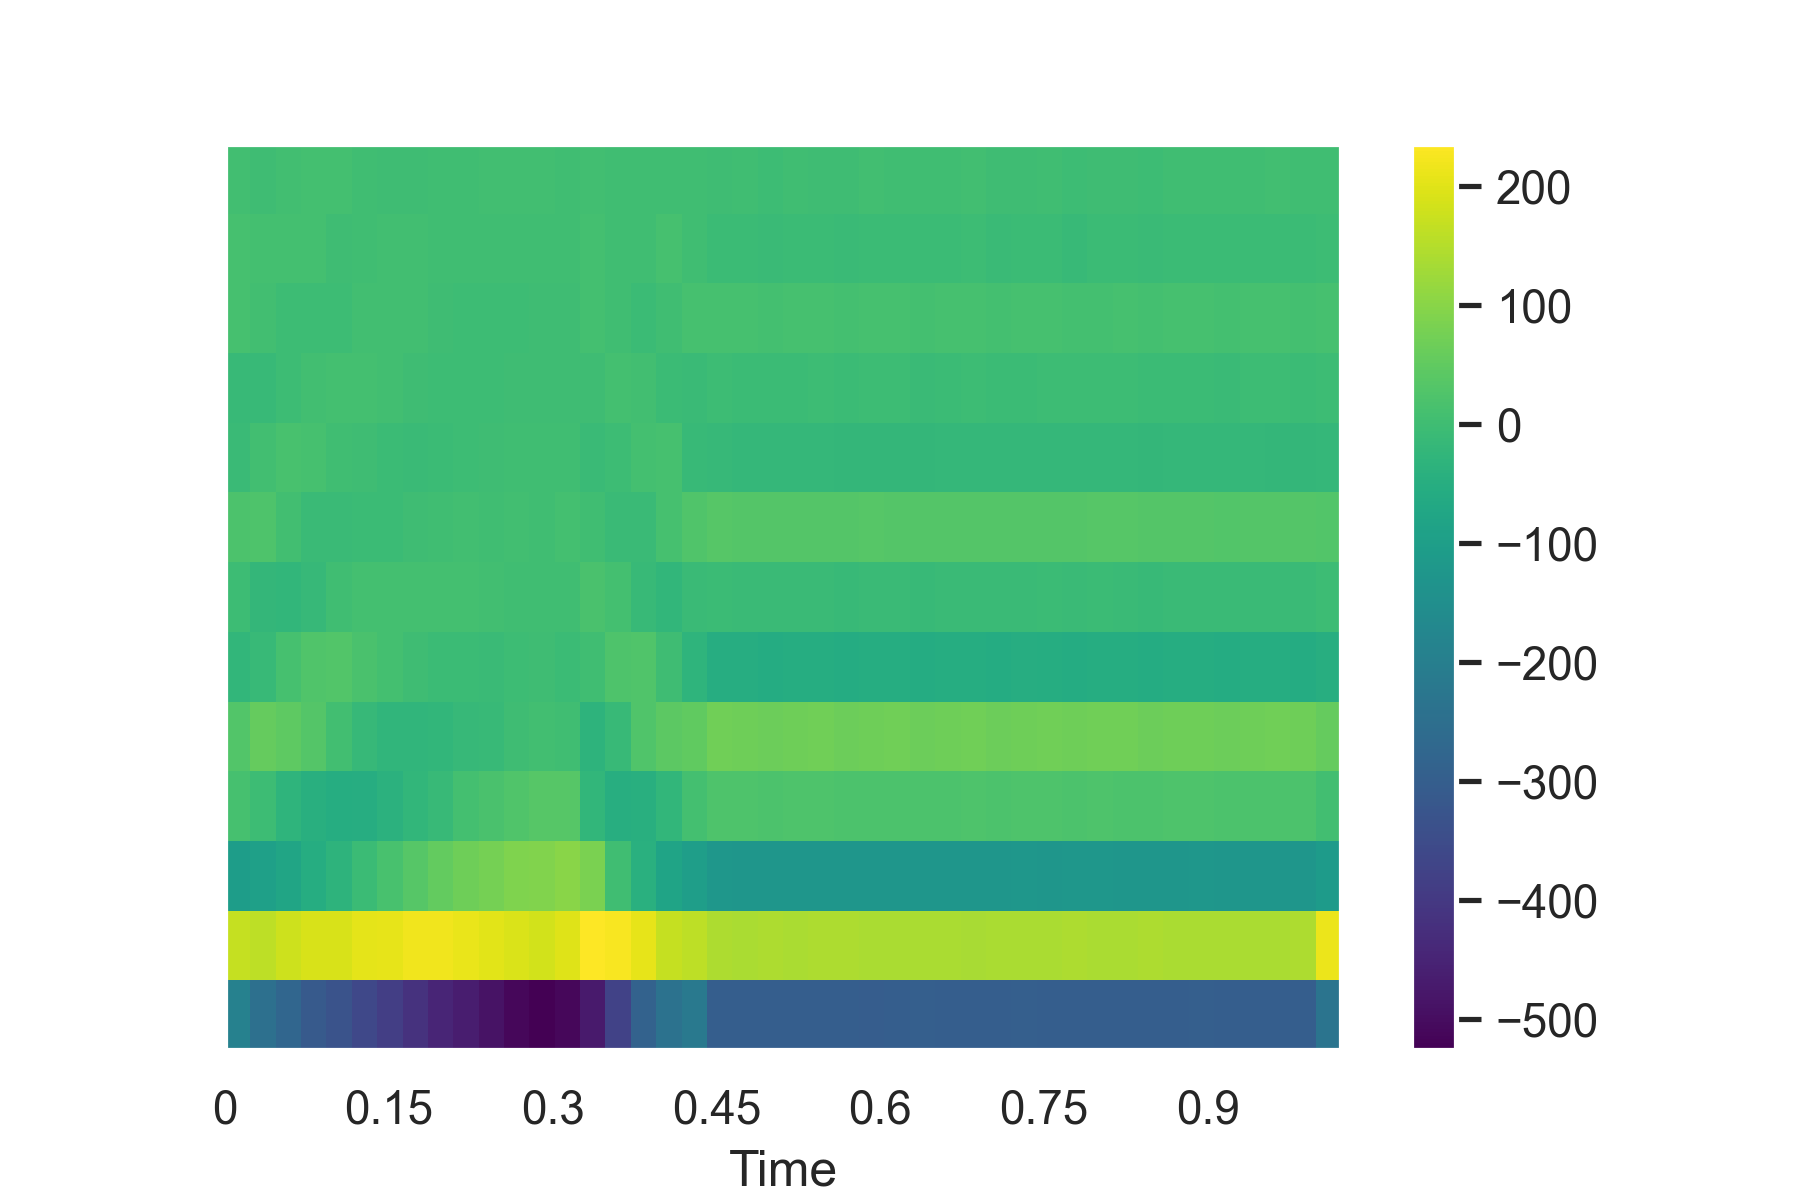
\includegraphics[width=\textwidth]{figures/inverse-synth/features_mfcc_example.png}
        \caption{MFCC}
    \end{subfigure}
    \begin{subfigure}[b]{0.45\textwidth}
        \centering
        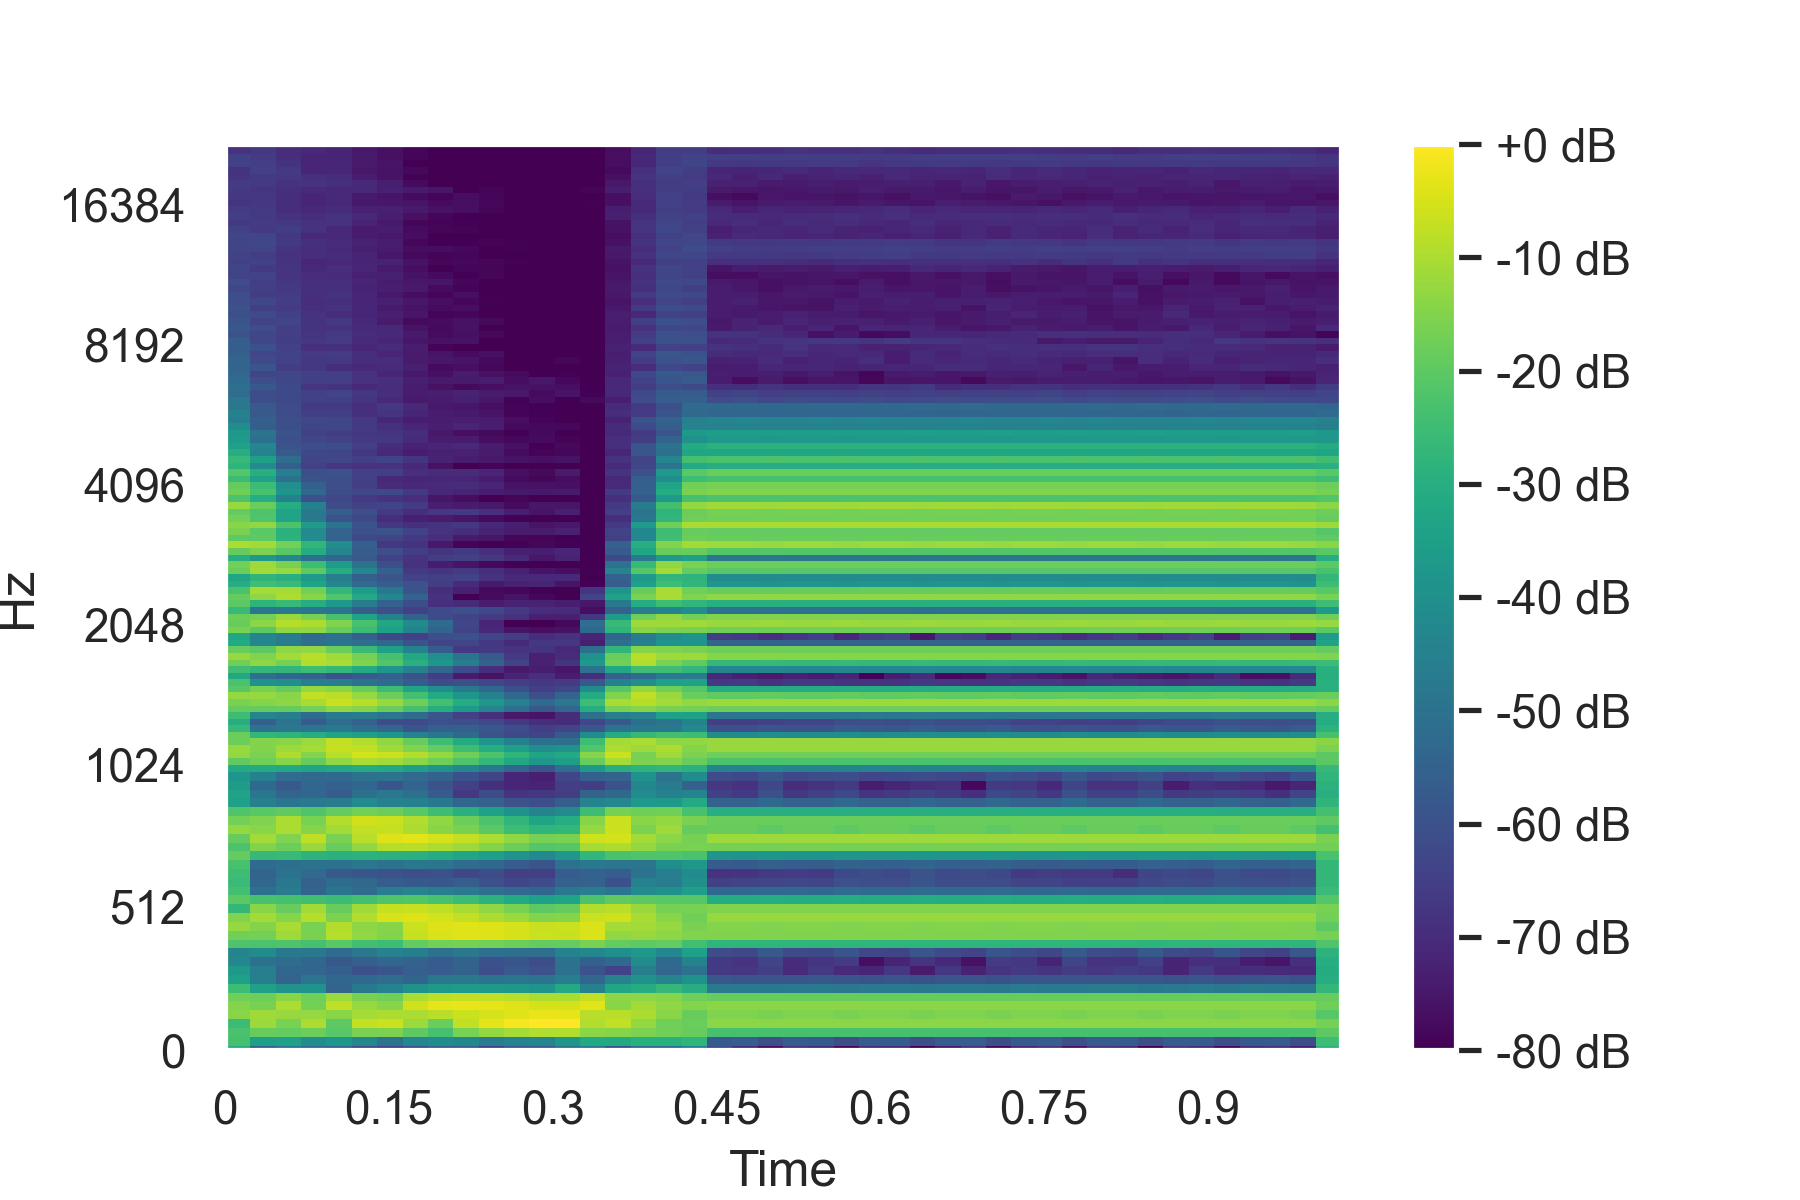
\includegraphics[width=\textwidth]{figures/inverse-synth/features_mel_example.png}
        \caption{Mel-Spectrogram}
    \end{subfigure}
    \caption{Audio representations generated for a single audio example in the dataset. The left figures shows a 13-band MFCC, and the right shows a log-scaled 128-band Mel-Spectrogram.}
    \label{fig:mfcc-mel-representations}
\end{figure}

\section{Deep Learning Models}
Eight different models were used in this experiment. Three recurrent neural networks (RNNs) derived from work by Yee-King \textit{et al.} \cite{yee2018automatic}, four convolutional neural networks (CNNs) derived from work by Barkan \textit{et al.} \cite{barkan2019inversynth}, and a baseline multi-layer perceptron (MLP) network, also from Yee-King \textit{et al.} \cite{yee2018automatic}. The RNN models use the time-series of MFCC features as input, the CNN models use the Mel-spectrogram images as input, and the MLP network uses a flattened version of the time-series MFCC features. All models output floating point value estimations for the nine synthesizer parameters. Because these output values can be any 32-bit floating point number (outputs are clipped to a $[0-1]$ range), this means that the models are solving a regression problem. The loss function used during training was the mean squared error (MSE) between the target parameter values $\textbf{y}$ and the predicted parameter values $\hat{\textbf{y}}$. The MSE is calculated as follows, where $N$ is the number of parameters:

\begin{equation}\label{equation:mse}
    \ell(\textbf{y}, \hat{\textbf{y}}) = \frac{\sum_{i \in N}{(y_i - \hat{y_i})^2}}{N}
\end{equation}

Ideally the loss would be calculated on audio produced by Dexed using the estimated parameters, however there are currently no available solutions for rendering audio using VST instruments within a deep learning model and including it in the the training loop. Recent work by Ramírez \textit{et al.} presented a solution for including audio effect plugins within a deep learning networks \cite{ramirez2021differentiable} which could also enable training on VSTis as well, however I leave that for future suggested work. 

Models were trained using an $Adam$ optimizer \cite{kingma2014adam} and hyperparameters for each model were optimized using a  Tree-structured Parzen Estimator (TPE), which has been shown to be an effective method for hyperparameter selection \cite{bergstra2011algorithms}. Early stopping was used during training for all models, this halted training if the validation loss stopped decreasing for a certain number of training epochs. The number of training epochs that early stopping waited before halting training is referred to as $patience$, and was selected based on results from hyperparameter optimization.

The following subsections describe each of the models that were included in this experiment. To find specific details on the implementation of each model see appendix \ref{appendix:spiegelib_models}.

% Maybe not important
%This is a natural way to approach the problem considering the continuous nature of the parameters exposed by a given synthesizer, and this is the approach taken by Yee-King \textit{et al.}. Conversely, Barkan \textit{et al.} framed the inverse synthesis problem as a classification problem by dividing each parameter into 16 classes, which meant that there would be $n*16$ classes, where $n$ is the number of parameters. Quantizing the parameter space into 16 discrete values per parameter 

\subsection{Multi-Layer Perceptron}
% Find cites for  the MLP?
Multi-Layer Perceptron (MLP) models, also referred to as a feedforward neural network, were the first and most simple types of neural networks. They contain one or more hidden layers containing neurons that are connected to each neuron in the preceding and proceeding layers. Because of fully connected nature of these layers, they are also referred to as dense layers. An MLP is included in this experiment as a baseline model to benchmark the other models againsts. The architecture for the MLP was derived from Yee-King \textit{et al.} \cite{yee2018automatic} and has three hidden layers containing 50, 40, and 30 neurons respectively. Each neuron utilizes a ReLu activation and the model contains 32k trainable parameters. It was trained using a learning rate of 0.001, a patience of 25 epochs, and a batch-size of 128.

\subsection{Recurrent Neural Networks}
% Find cites for these different networks??
Three different Recurrent Neural Networks (RNNs) derived from work by Yee-King \textit{et al.} \cite{yee2018automatic} were used in this experiment:
\begin{itemize}
    \item \textit{LSTM:} The first is an RNN with three LSTM layers, each containing 64 units, followed by a dropout layer with frequency of 0.2 and a fully connected output layer. It contains 86.6k trainable parameters. This is a modified version of the model used by Yee-King, the number of units for each LSTM and the rate of the dropout were both selected through hyperparameter optimization; the main difference is that this model uses only 64 units in each LSTM as opposed to 100, meaning that the tuned model contains less trainable parameters. This model was trained with a learning rate of 0.001, early-stopping patience of 30 epochs, and a batch-size of 64.
    \item \textit{LSTM++:} This model is the same LSTM++ model proposed by Yee-King. Each LSTM in the bi-directional layer contains 128 units. A dropout with a rate of 0.2 follows the bi-directional layer. This is then projected down to 64 dimensions using a dense layer with an exponential linear unit (ELU) activation. Six highway layers follow this, also with ELU activations. The highway layers perserve the dimensionality of the input. The final highway layer is connected to the output with a fully connected layer containing an ELU activation. This model contains 212k trainable parameters and was trained using a learning rate of 0.001, early-stopping patience of 30, and a batch-size of 32.
    \item \textit{5-LSTM++:} This model is an attempt to optimize the previous LSTM++ model for the specific problem. The main different between this model and the LSTM++ is that it only contains five highway layers, and each highway layer is only 32 dimensions. Therefore, the capacity of this model is less than that of the LSTM++; it contains 164.5k trainable parameters. The dropout layer also operates at a higher dropout rate of 0.5. This model was trained using the same learning rate and early-stopping patience as the LSTM++, but with a larger batch-size of 128.
\end{itemize}

\subsection{Convolutional Neural Networks}
Four different convolution networks based on models proposed by Barkan \textit{et al.} were used \cite{barkan2019inversynth}. In their work, Barkan \textit{et al.} experimented with seven different CNN models that used a log STFT spectrogram for input. They found that the model with the most capacity, a model with 6 CNN layers and 2.3M trainable parameters, performed the best in their experiments. All the other spectrogram based models that they experimented with had 1.2M trainable parameters and had between one to six convolutional layers. They also use strided convolutions as opposed to the more traditional max pooling approach to downsample between layers \cite{goodfellow2016deep}. The 6-layer and 5-layer networks proposed by Barkan \textit{et al.} were used for this experiment, these models were called \textit{Conv6} and \textit{Conv5} respectively. Early experiments showed that these models were prone to overfitting on the Dexed parameter estimation dataset and two derivative models with less capacity were developed for this experiment, these models were called \textit{Conv6s} and \textit{Conv5s}, where the appended "s" stands for "small". The Conv6 and Conv5 models were modified by reducing the size of the filters in each convolutional layer to produce the smaller models. Both the Conv6 and Conv5 networks contained 1.1M trainable parameters, the Con6s model contained 686k trainable parameters, and the Conv5s model contained 600k trainable parameters. 

Hyperparameter optimization with TPE was used to further refine these models. Model parameters that were included in the optimization were the depth and size of the fully connected layers that were inserted before the output, whether or not to include batch-normalization between the convolutional layers, and the amount of dropout to include before and between each of fully connected layers. Based on the optimization trials, two fully connected layers of size 512 were selected, batch normalization was included, and a dropout with rate 0.2 was selected. These modifications were applied to all four of the convolution models. Figure \ref{fig:conv5s} shows a diagram of the Conv5s architecture, without the batch normalization and dropout layers.

\begin{figure}[ht]
    \centering
    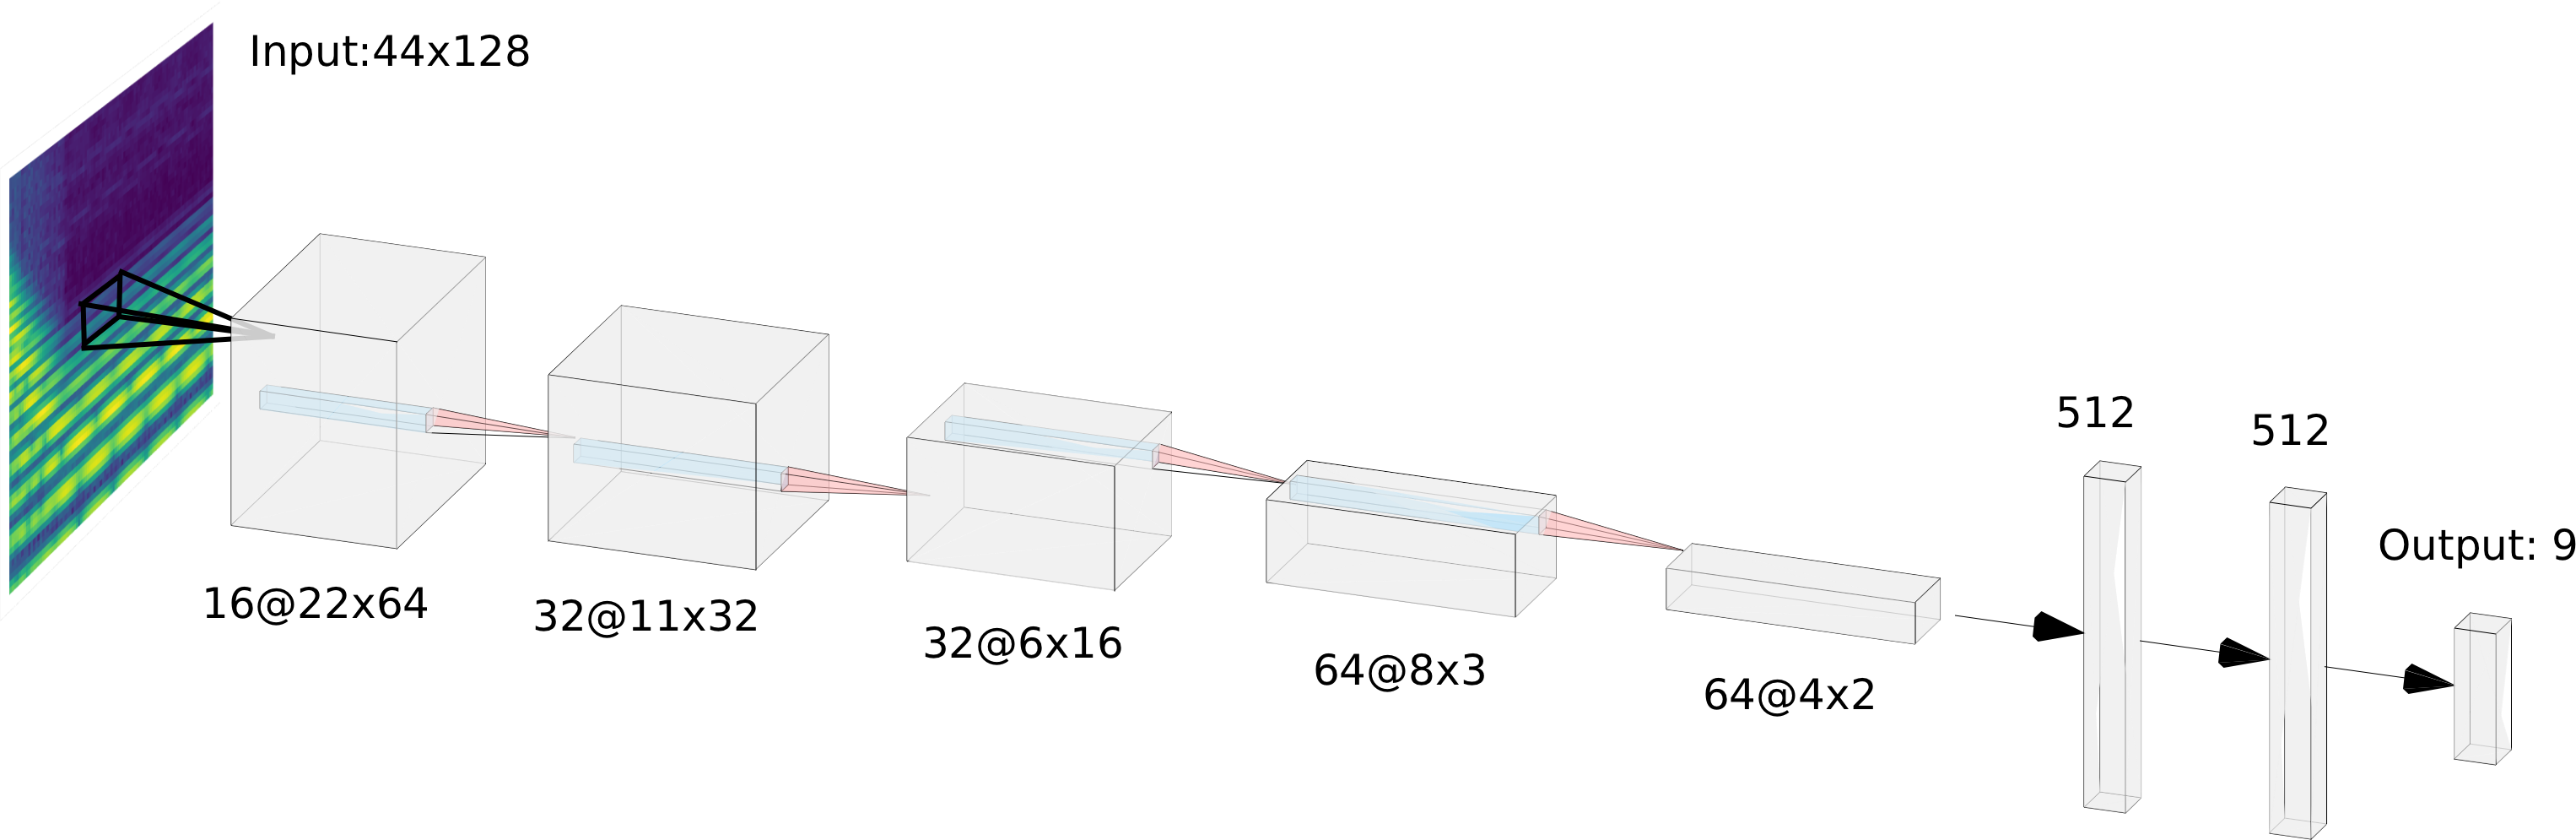
\includegraphics[width=0.99\textwidth]{figures/inverse-synth/CONV5s_Diagram.png}
    % Add a bit more description in this figure
    \caption{Network diagram of the Conv5s CNN. This model accepts a Mel-spectrogram as input and contains five 2D convolutional layers followed by two dense layers. The output layer is predicted synthesizer parameters.}
    \label{fig:conv5s}
\end{figure}

During initial experiments all of the models (especially the models with more capacity) began to overfit during training after about 50 epochs. A learning rate schedule was introduced in an attempt to address this and allow the models to train for longer. An inverse time-decay scheduler was included that reduced the learning rate according to the following equation:

\begin{align}
    \eta_i = \frac{\eta_0}{1 + \lambda\frac{i}{T}}
\end{align}

Where $\eta_i$ is the learning rate at training step $i$, $\eta_0$ is the initial learning rate, $\lambda$ is the decay rate, and $T$ is the decay steps. For this experiment $\eta_0=0.001$, $\lambda=1.0$, and $T$ was set to be equivalent to 50 epochs, which means that the decay rate decreased by a factor of two by 50 epochs into training. All the CNNs were trained using this learning schedule, an early-stopping patience of 20, and a batch-size of 128. 

\subsection{Training Results}
All the models were allowed to train until the early-stopping criteria was triggered. The 5-LSTM++ model trained for the most number of epochs (151 epochs), and the Conv5 model trained for the least (60 epochs). Models were trained on an NVIDIA RTX 2080 super GPU, training time ranged between X for the X model, and Y for the Y model. All training times are listed in appendix \ref{appendix:training-times}.

Validation loss at each training epoch is shown in figure \ref{fig:training-loss} and plots for all models plotted against their respective training loss are provided in appendix \ref{appendix:training-loss}. These plots show a much smoother curve for all the LSTM models and the MLP compared to the convolutional networks. Even with the learning rate schedule the two full-sized Conv6 and Conv6 networks began to overfit before 50 epochs, and the Conv5 network shows quite severe signs of overfitting after 50 epochs. Overall, the LSTM model achieved the lowest validation loss, finishing the last epoch with an error of 0.0495.

\begin{figure}[ht]
    \centering
    \begin{subfigure}[b]{0.45\textwidth}
        \centering
        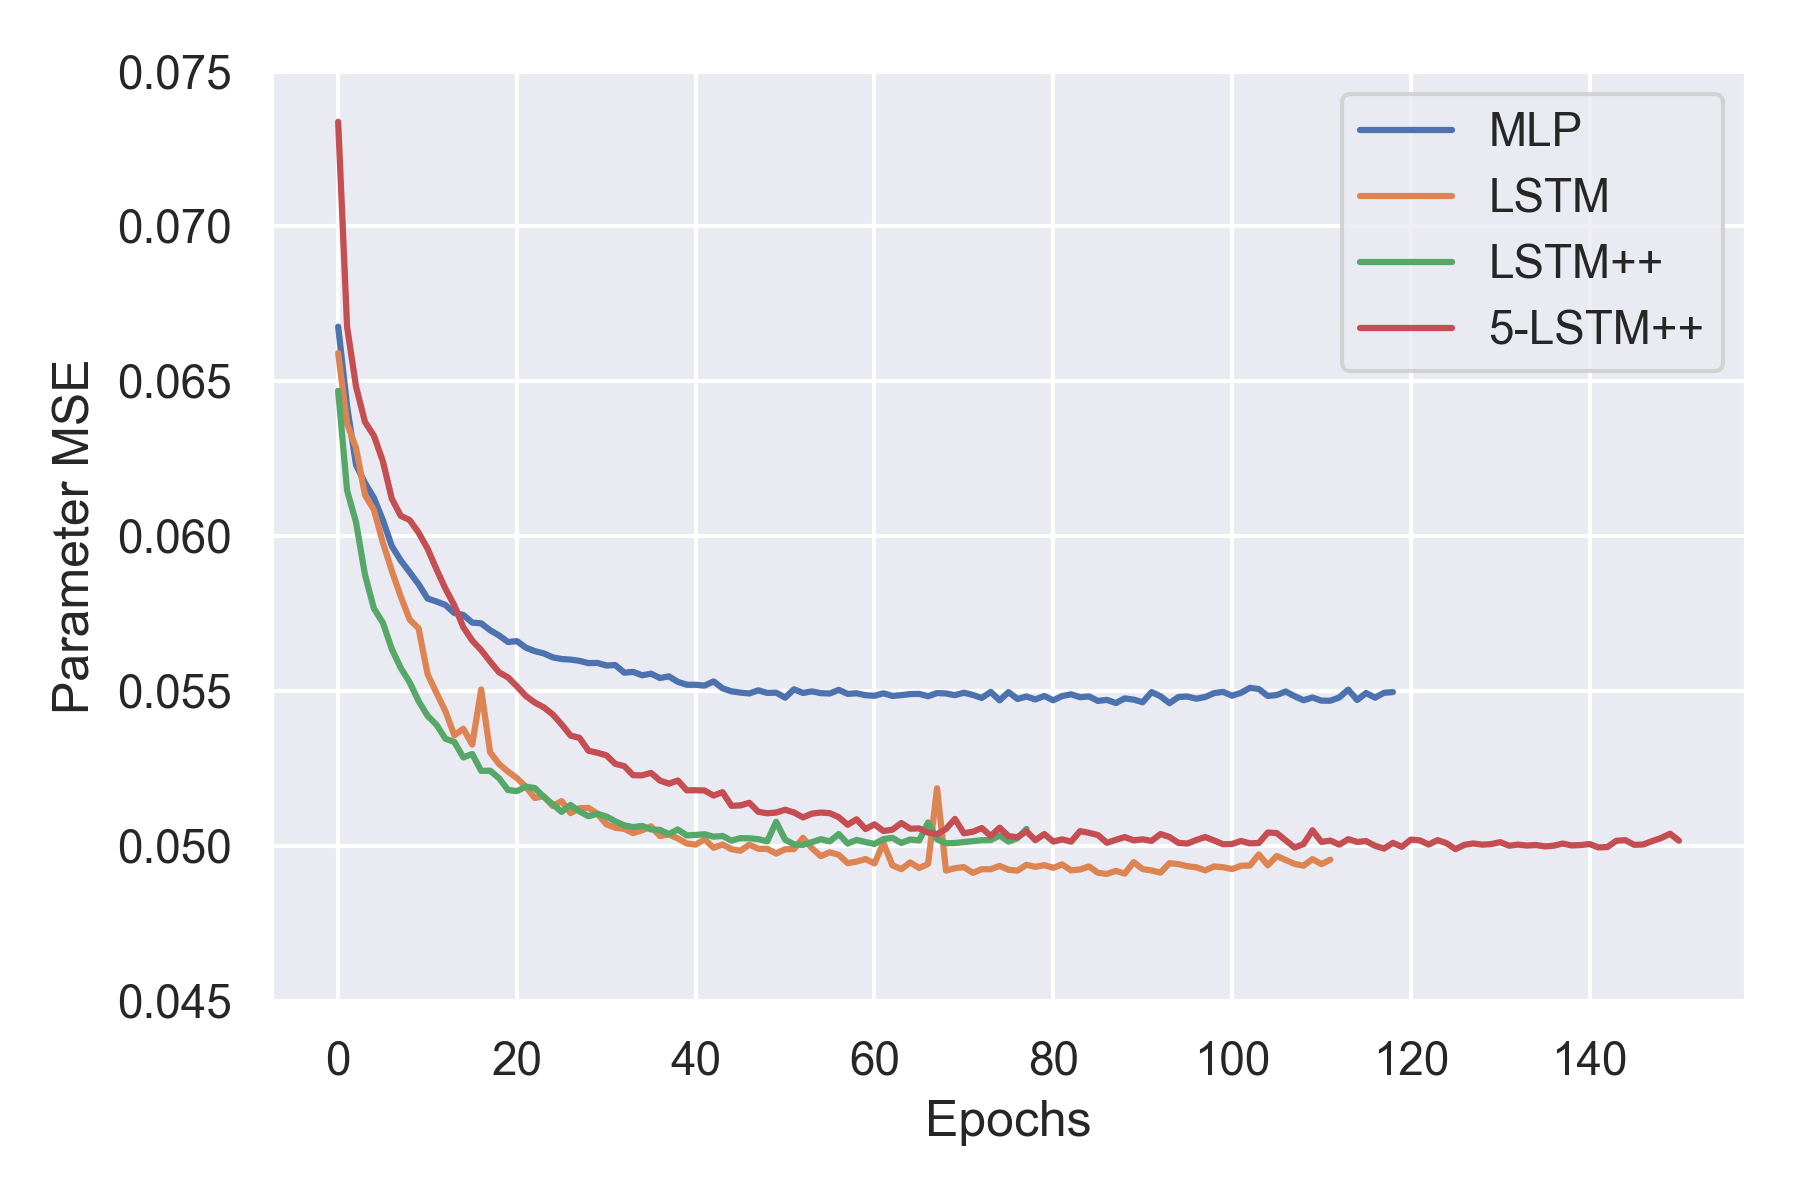
\includegraphics[width=\textwidth]{figures/inverse-synth/lstm-loss.png}
    \end{subfigure}
    \begin{subfigure}[b]{0.45\textwidth}
        \centering
        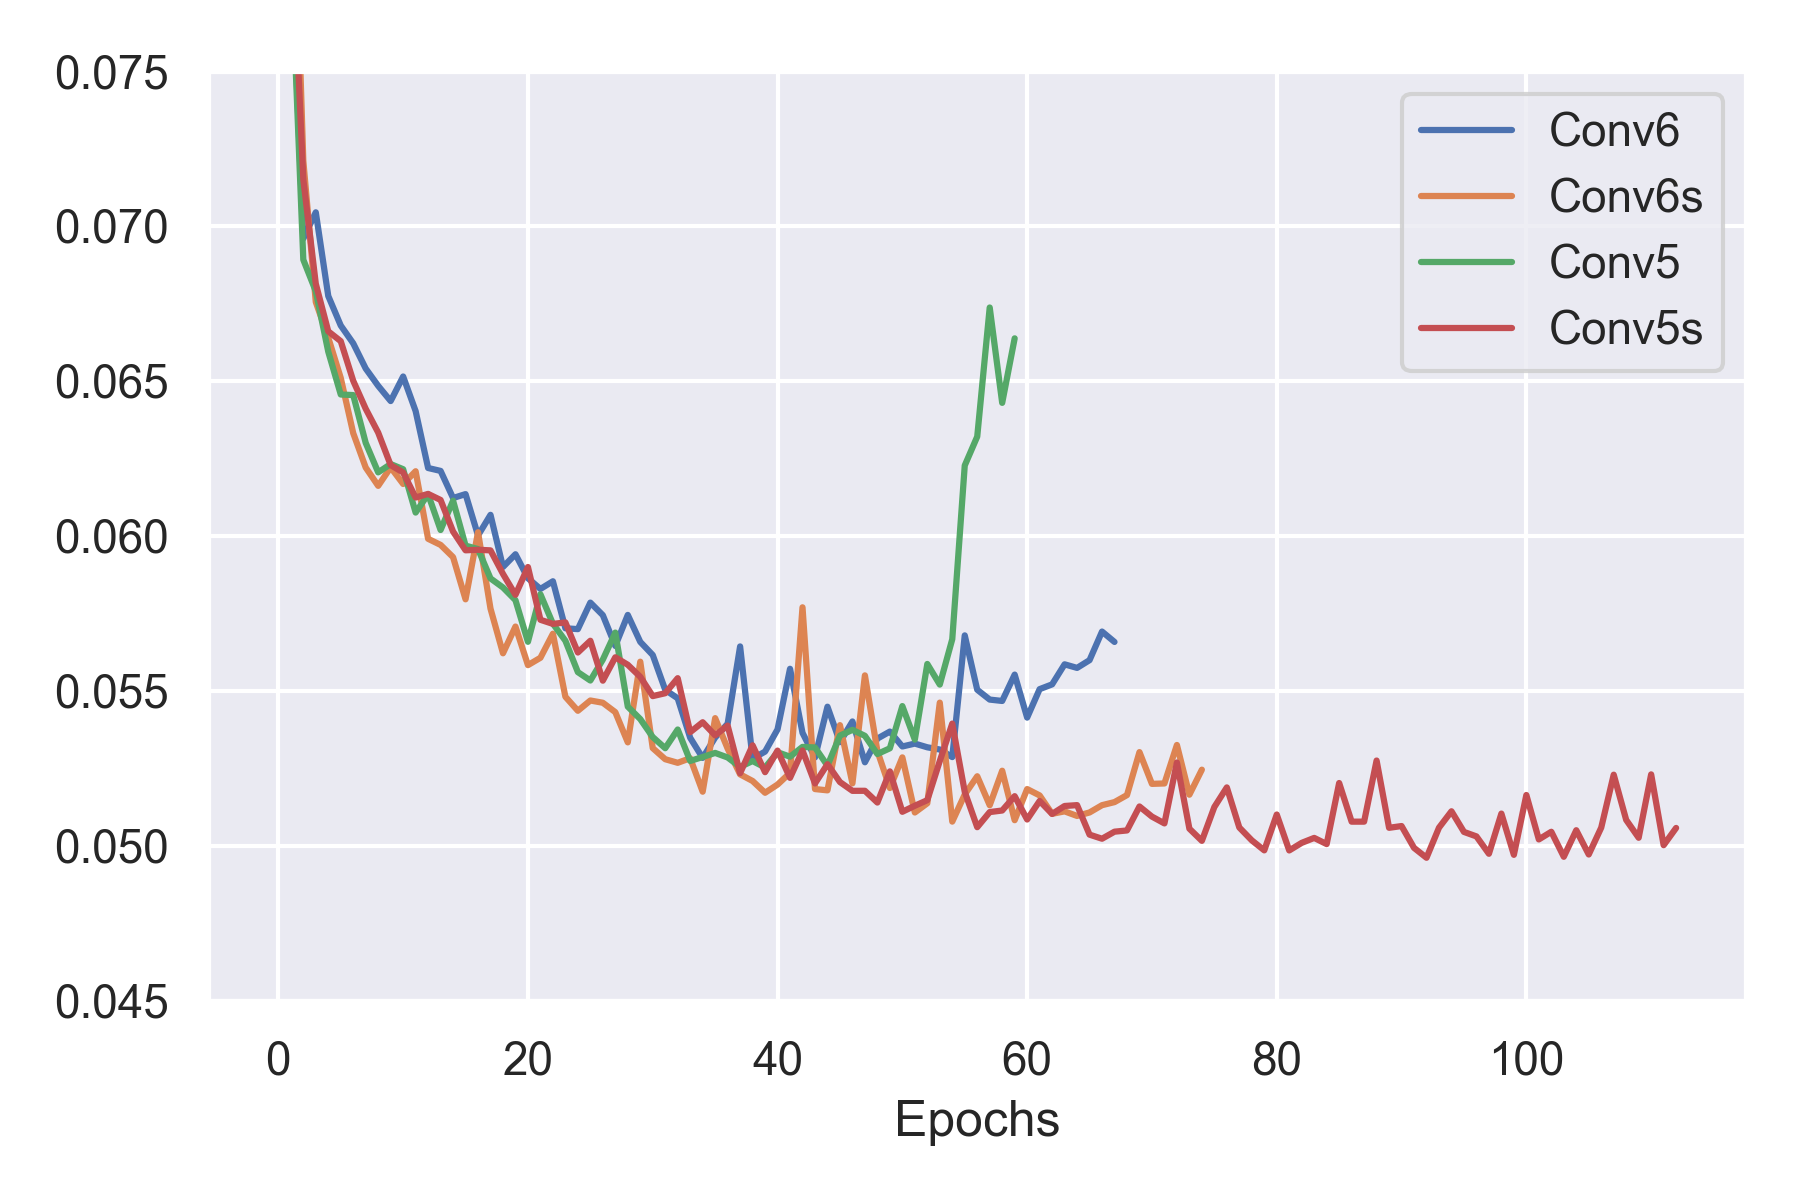
\includegraphics[width=\textwidth]{figures/inverse-synth/conv-loss.png}
    \end{subfigure}
    \caption{Validation loss during training for all the deep learning models. Models are split into two separate figures for visibility: the MLP and LSTM models are on the left, and the CNN models are on the right.}
    \label{fig:training-loss}
\end{figure}

\section{Genetic Algorithms}
Two different GAs were used: a basic single-objective GA and a multi-objective NSGA III. The multi-ojective GA was derived from work conducted by Tatar \textit{et al.} \cite{tatar2016automatic} that used the algorithm to automatically tune the parameters of a Teenage Engineering OP-1\footnote{\url{https://teenage.engineering/products/op-1}} synthesizer. In the case of the GAs the $fitness$ is easily computed directly on the audio rendered from $Dexed$. During each iteration of the algorithm, individuals of the population (whose genotype are synthesizer parameters) are rendered using Dexed, and the phenotype is produced by generating an audio representation from the resulting audio.

\subsection{Fitness}
In the case of the basic GA the $fitness$ is computed as the mean absolute error (MAE) between 13-band MFCCs from the target and the individual. The MFCCs were calculated using a frame-size of 2048 samples and a hop-size of 1024 samples. MAE is calculated as follows, here $N$ is the number of features, $y$ is the target, and $\hat{y}$ is the predicted individual:

\begin{equation}\label{equation:mae}
    \text{MAE} = \frac{\sum_{i \in N}{|y_i - \hat{y}_i|}}{N}
\end{equation}
 
 Three different metrics were used for evaluating the $fitness$ of an individual for the NSGA-III algorithm, MAE between: 1) a 13-band MFCC, 2) magnitude spectrum from an FFT, and 3) a set of spectral features. The MFCCs were calculated using a frame-size of 2048 samples and hop size of 1024 samples. The FFT was calculated over the entire input audio, 1 second at 44,100 samples/second. For the spectral features, five different features were calculated: centroid, bandwidth, contrast across seven subbands, flatness, and rolloff. Each feature was calculated using a frame-size of 2048 samples and a hop-size of 1024 samples. The time series of audio features was summarized using the mean and variance. This resulted in a feature vector of size 22.
 
 \subsection{Time Complexity}
 The quality of the result that can be produced by a GA is generally related to the amount of time that the algorithm is allowed to run for. While there is no guarantee that the optimal solution will be found, and the optimization may get stuck in a local minima, allowing the the algorithm to run for longer will give the GA a higher likelihood of converging on a quality solution. Tatar \textit{et al.} allowed their NSGA-III run for 5 hours on a 50-core computer, which lead to results that were competitive against human sound designers. The synthesizer programming task in their problem was much more complex than the problem presented in this experiment. Initial experiments showed both GAs were able to perform well when allowed to run for 100 generations with a population of 300 individuals. For the NSGA this took about 20 minutes on a late 2013 MacBook Pro. Although this time is much better than 5hrs, this still presented a limitation to the number of target examples that could be used for evaluation. Also, 20 minutes is still too long for the method to be practical in a music production context. A more severely constrained test was designed to see if the GAs still remained superior to the deep learning approaches. Each GA was allowed to run for only 25 generations using a population of 100 individuals. With these constraints the runtime was approximately 75 seconds for the NSGA-III and 41 seconds for the basic GA.
 
 \subsection{Mutation and Crossover}
 The remaining hyperparameters that control each GA are the rate of mutation and the rate of crossover. The rate of mutation sets the likelihood that a genotype is randomly modified. The rate of mutation was 30\% for the basic GA and 50\% for the NSGA-III. Rate of crossover set the likelihood that an individual is combined with another individual to create an new "child" individual. The rate of crossover for both GAs was set to 50\%.


% Both genetic algorithms were run for 100 generations for each sound target. The basic GA and NSGA used population sizes of 300 and 100 individuals respectively. 

%Figure \ref{fig:nsga_fitness} shows the minimum spectral error achieved by an individual during each iteration of the NSGA algorithm on one of the target sounds. The plot shows a period of rapid improvement during early iterations, with some short periods of stagnation, followed by longer periods where the algorithm is unable to find an individual that is an improvement over those in the current population.

% TODO: Add in the other population generation plots for each objective

% \begin{figure}[ht]
% \begin{center}
% 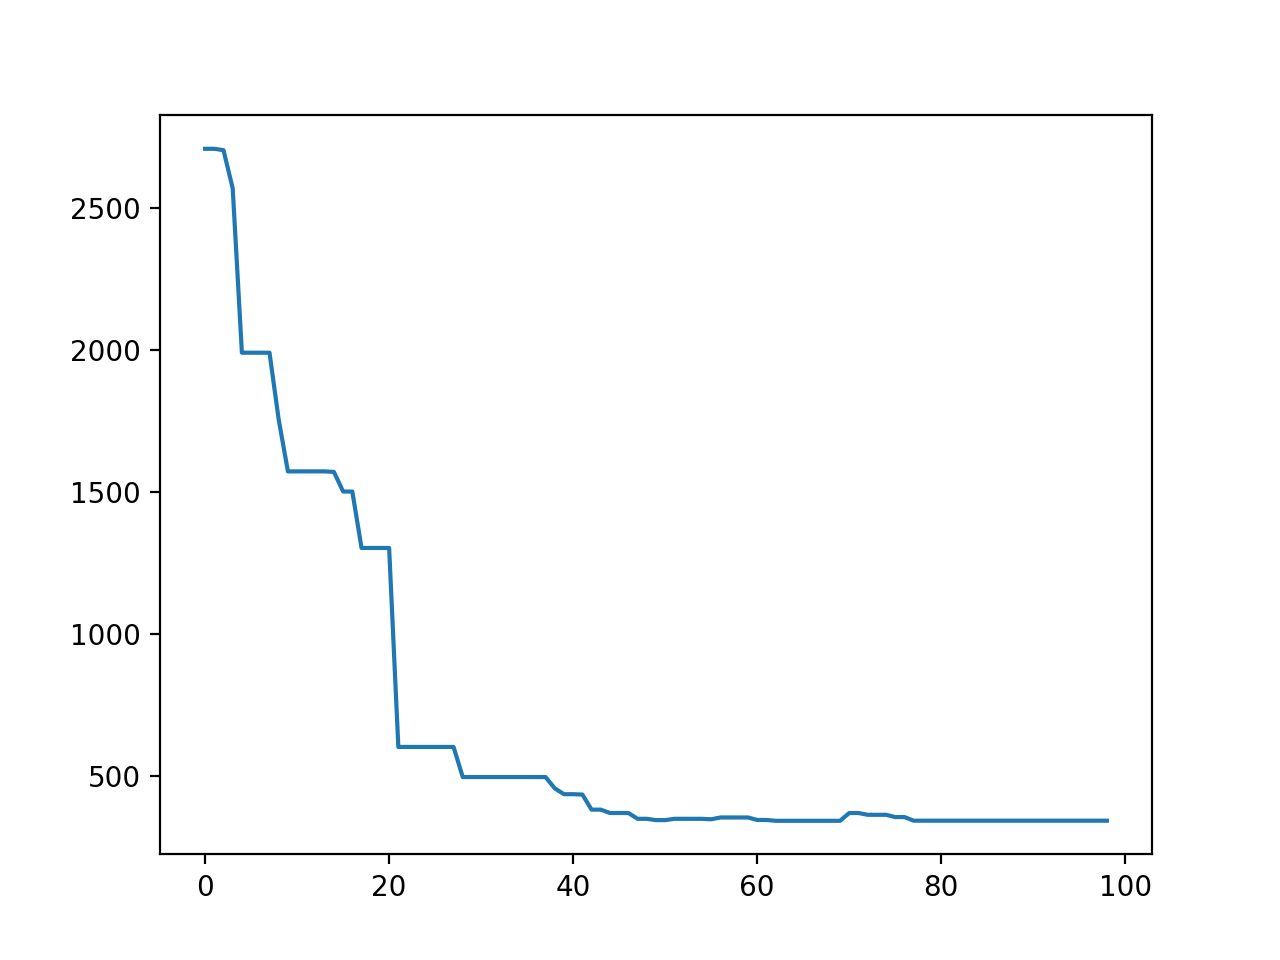
\includegraphics[width=0.7\columnwidth]{nsga_target_15_FFT.png}
% \caption{Minimum FFT MAE in the population at each generation to target sound 15 for NSGA III estimator.}
% \label{fig:nsga_fitness}
% \end{center}
% \end{figure}

\section{Evaluation}
\label{sec:inverse-synth-eval}

Evaluation was carried out by measuring the ability of each technique to accurately perform inverse synthesis on a dataset of testing sounds. A dataset with 250 examples was created for this purpose using the same technique for rendering sounds described earlier in this chapter (see \S\ref{sec:dataset-generation}). The same nine parameter subset of sounds were used for the test dataset; using sounds generated from this synthesizer configuration means that an exact match for inverse synthesizer is possible, which provides a known baseline for comparing each of the methods. Each of the 10 different techniques were were run on each of the 250 target test sounds and parameters estimated. Predicted audio was rendered using Dexed and the the resulting audio and parameter pairs were saved for evaluation. The results were evaluated quantitatively using three different metrics: 1) MFCC MAE,  2) Log Spectral Distance (LSD), 3) Parameter MAE. The first two metrics evaluate on the audio produced by rendering the estimated parameters whereas the third metric evaluates the accuracy of the parameters themselves. In the case of inverse synthesis we are most interesting in evaluating how closely an estimated synthesizer patch can reproduce a target sound, which would be evaluated by the auditory metrics best. The parameter metric provides insight into how each technique is selecting parameters and helps to elucidate the strengths and weaknesses of each approach. Each metric is described in more detail below and all the results are summarized in table \ref{tbl:objective_resuls}.

\begin{table}[ht]
\centering
\begin{tabular}{r|ccc}
\toprule
% {} & \multicolumn{2}{c}{MFCC MAE} & \multicolumn{2}{c}{LSD} & \multicolumn{2}{c}{Parameter MAR} \\
{} & MFCC & LSD & Parameter \\
\midrule
MLP      &       $8.3 \pm 7.8$ &     $87.6 \pm 13.8$ &  $0.188 \pm 0.048$ \\
\midrule
LSTM     &       $6.6 \pm 4.7$ &     $84.8 \pm 11.8$ &  $\mathbf{0.171 \pm 0.053}$ \\
5-LSTM++ &       $7.2 \pm 5.2$ &     $87.2 \pm 11.0$ &  $0.173 \pm 0.051$ \\
LSTM++   &       $6.8 \pm 5.8$ &     $85.8 \pm 11.2$ &  $0.172 \pm 0.051$ \\
\midrule
Conv6    &       $8.2 \pm 8.0$ &     $87.5 \pm 13.3$ &  $0.189 \pm 0.052$ \\
Conv6s   &       $8.6 \pm 7.9$ &     $87.9 \pm 12.8$ &  $0.181 \pm 0.054$ \\
Conv5    &      $11.4 \pm 9.9$ &     $91.4 \pm 19.4$ &  $0.203 \pm 0.065$ \\
Conv5s   &       $7.3 \pm 6.3$ &     $86.1 \pm 12.4$ &  $0.180 \pm 0.052$ \\
\midrule
GA       &       $4.9 \pm 3.2$ &     $83.1 \pm 12.3$ &  $0.281 \pm 0.085$ \\
NSGA     &       $\mathbf{2.0 \pm 2.2}$ &     $\mathbf{73.2 \pm 17.9}$ &  $0.243 \pm 0.080$ \\
\bottomrule
\end{tabular}
\caption{Summary of quantitative results for inverse synthesis evaluation. The values in bold are the scores with the lowest mean for that metric.}
\label{tbl:objective_resuls}
\end{table}

\subsection{MFCC Error}
The MFCC error is calculated by computing the mean absolute error between MFCCs from a target audio and a prediction. Yee-King \textit{et al.} \cite{yee2018automatic} also used MFCCs to evaluate the quality of predicted sounds, however they used the euclidian distance between MFCCs as opposed to MAE. The MAE was used here as it showed results in a range that was easier compare. It also provides an interesting comparison to the Log Spectral Distance that was also included. [Appendex X shows results for MFCC evaluation using the Euclidian Distance]. For this evaluation, MFCCs were caclulated using a frame size of 2048 and a hop-size of 512. Figure \ref{fig:mfcc-mae} shows a boxplot graph comparing all the techniques using this metric, ordered by the mean. There is quite high variance for all of the techniques and quite a few outliers with high error, even for the best techniques. However, based on the mean error, both the GAs performed the best and the NSGA was overall the best technique. Out of the deep learning models the LSTM models all performed the best, with the LSTM performing the best followed by the LSTM++.

\subsection{Log Spectral Distance}
The log spectral distance (LSD) is a distance metric that is calculated between to power spectrums to quantify difference. It was used by Masuda and Saito as a fitness objective in a genetic algorithm for inverse synthesis \cite{masudo2021quality}. This metric is included to add more depth to the audio evaluation. Masuda and Saito identified a the limitations with calculating error between synthesized sounds using MFCC, particularly with the ability of MFCC to capture specific frequency information as opposed to just the shape of the spectral envelope. LSD provides a more robust evaluation on the spectrograms of the results.  LSD is calculated as:

\begin{equation}
    LSD(P, \hat{P}) = \sqrt{\sum_{\omega}10\text{log}_{10}\left( \frac{P(\omega)}{\hat{P}(\omega)} \right)^2}
\end{equation}

Where $P$ is a target power spectrum, $\hat{P}$ is the power spectrum of a predicted sound, and $\omega$ is a frequency bin. Power spectrums were calculated using a STFT with an FFT size of 1024 samples and a hop-size of 512 samples. The average value of LSD over frames is used as the final evaluation metric in this evaluation. Lower values for LSD indicate a closer match. Figure \ref{fig:lsd} shows a boxplot graph comparing the results of this evaluation. Again, the variance is quite high among all the techniques. Based on the mean LSD, the ranking of each of the techniques is almost identical to the results obtained from the MFCC evaluation, except that the Conv6 model is now ranked higher than the MLP model. The NSGA algorithm is again ranked most highly based on this metric and has several outliers with smaller distances.

\subsection{Parameter Error}
This metric measures the mean absolute error (MAE) between the parameter values from a target and a prediction. In related work, Barkan \textit{et al.} included this metric to evaluate the distance between target and estimated synthesizer parameters, it is include here for the same reason. Figure \ref{fig:param-mse} shows a boxplot graph comparing the results of this evaluation. In terms of mean parameter accuracy across testing dataset, all the deep learning models outperformed both of the GAs. All the LSTM based models were in the top three models, with the LSTM performing overal the best.

In addition to calculating the MAE over all nine parameters for each target-prediction pair, the absolute error between individual parameters was calculated. This metrics provides insight into how each technique handled the various parameters, as well as specific aspects of the synthesizer programming task, specific the programming of the envelope generator and the tuning of the operator pitch. The frequency and tuning parameters affect the distribution of the harmonics in the frequency domain, whereas the envelope generator is related to the temporal aspect of the sound and how the frequencies evolve over time.



\begin{figure}[p]
    \centering
    \begin{subfigure}[b]{0.99\textwidth}
        \centering
        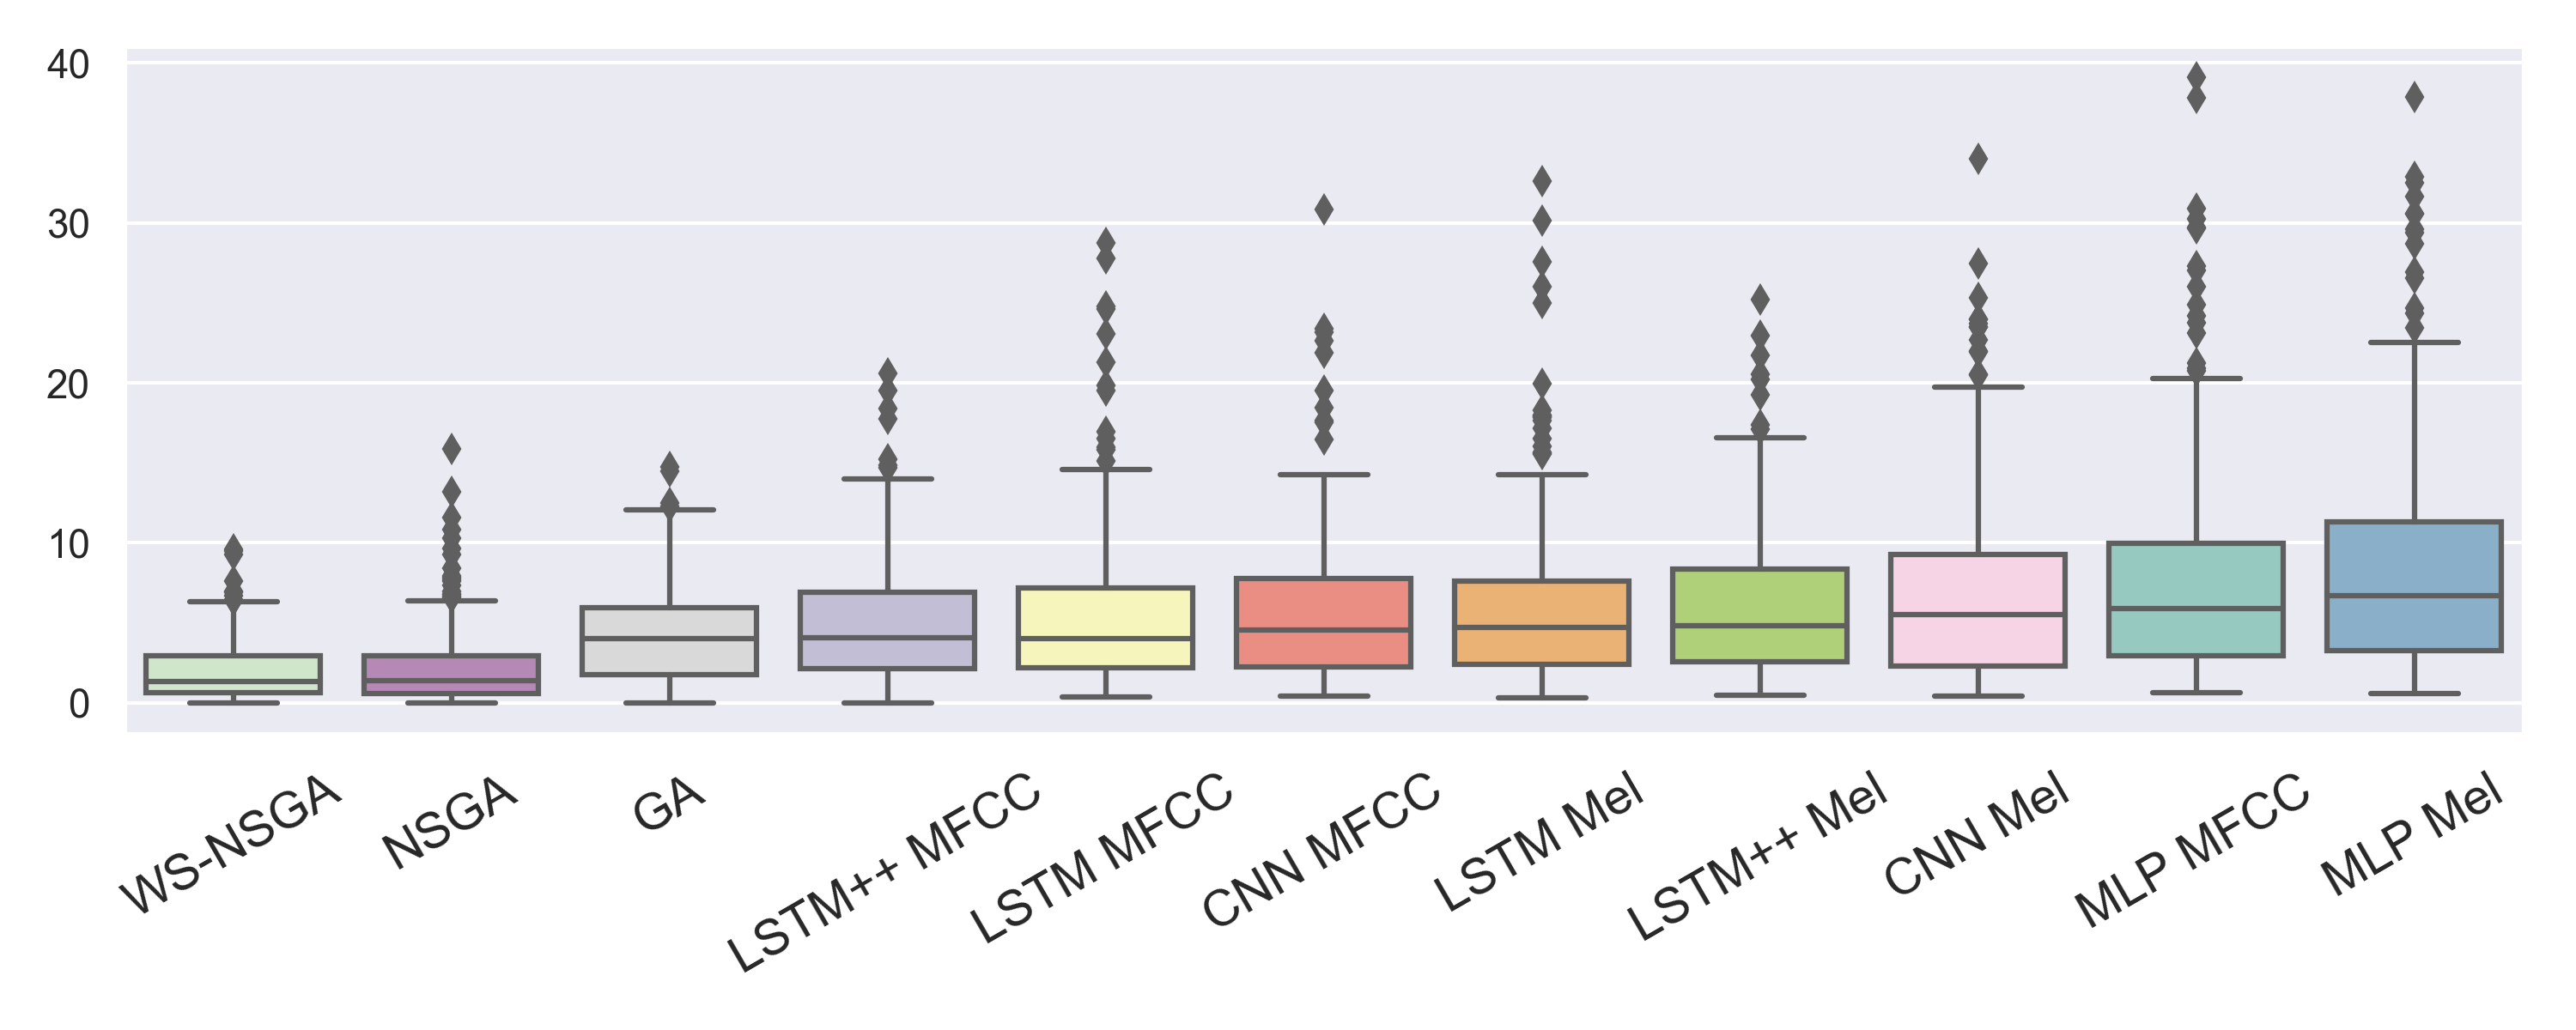
\includegraphics[width=\textwidth]{figures/inverse-synth/mfcc_mae_boxplot.png}
        \caption{MFCC MAE}
        \label{fig:mfcc-mae}
    \end{subfigure}
    \begin{subfigure}[b]{0.99\textwidth}
        \centering
        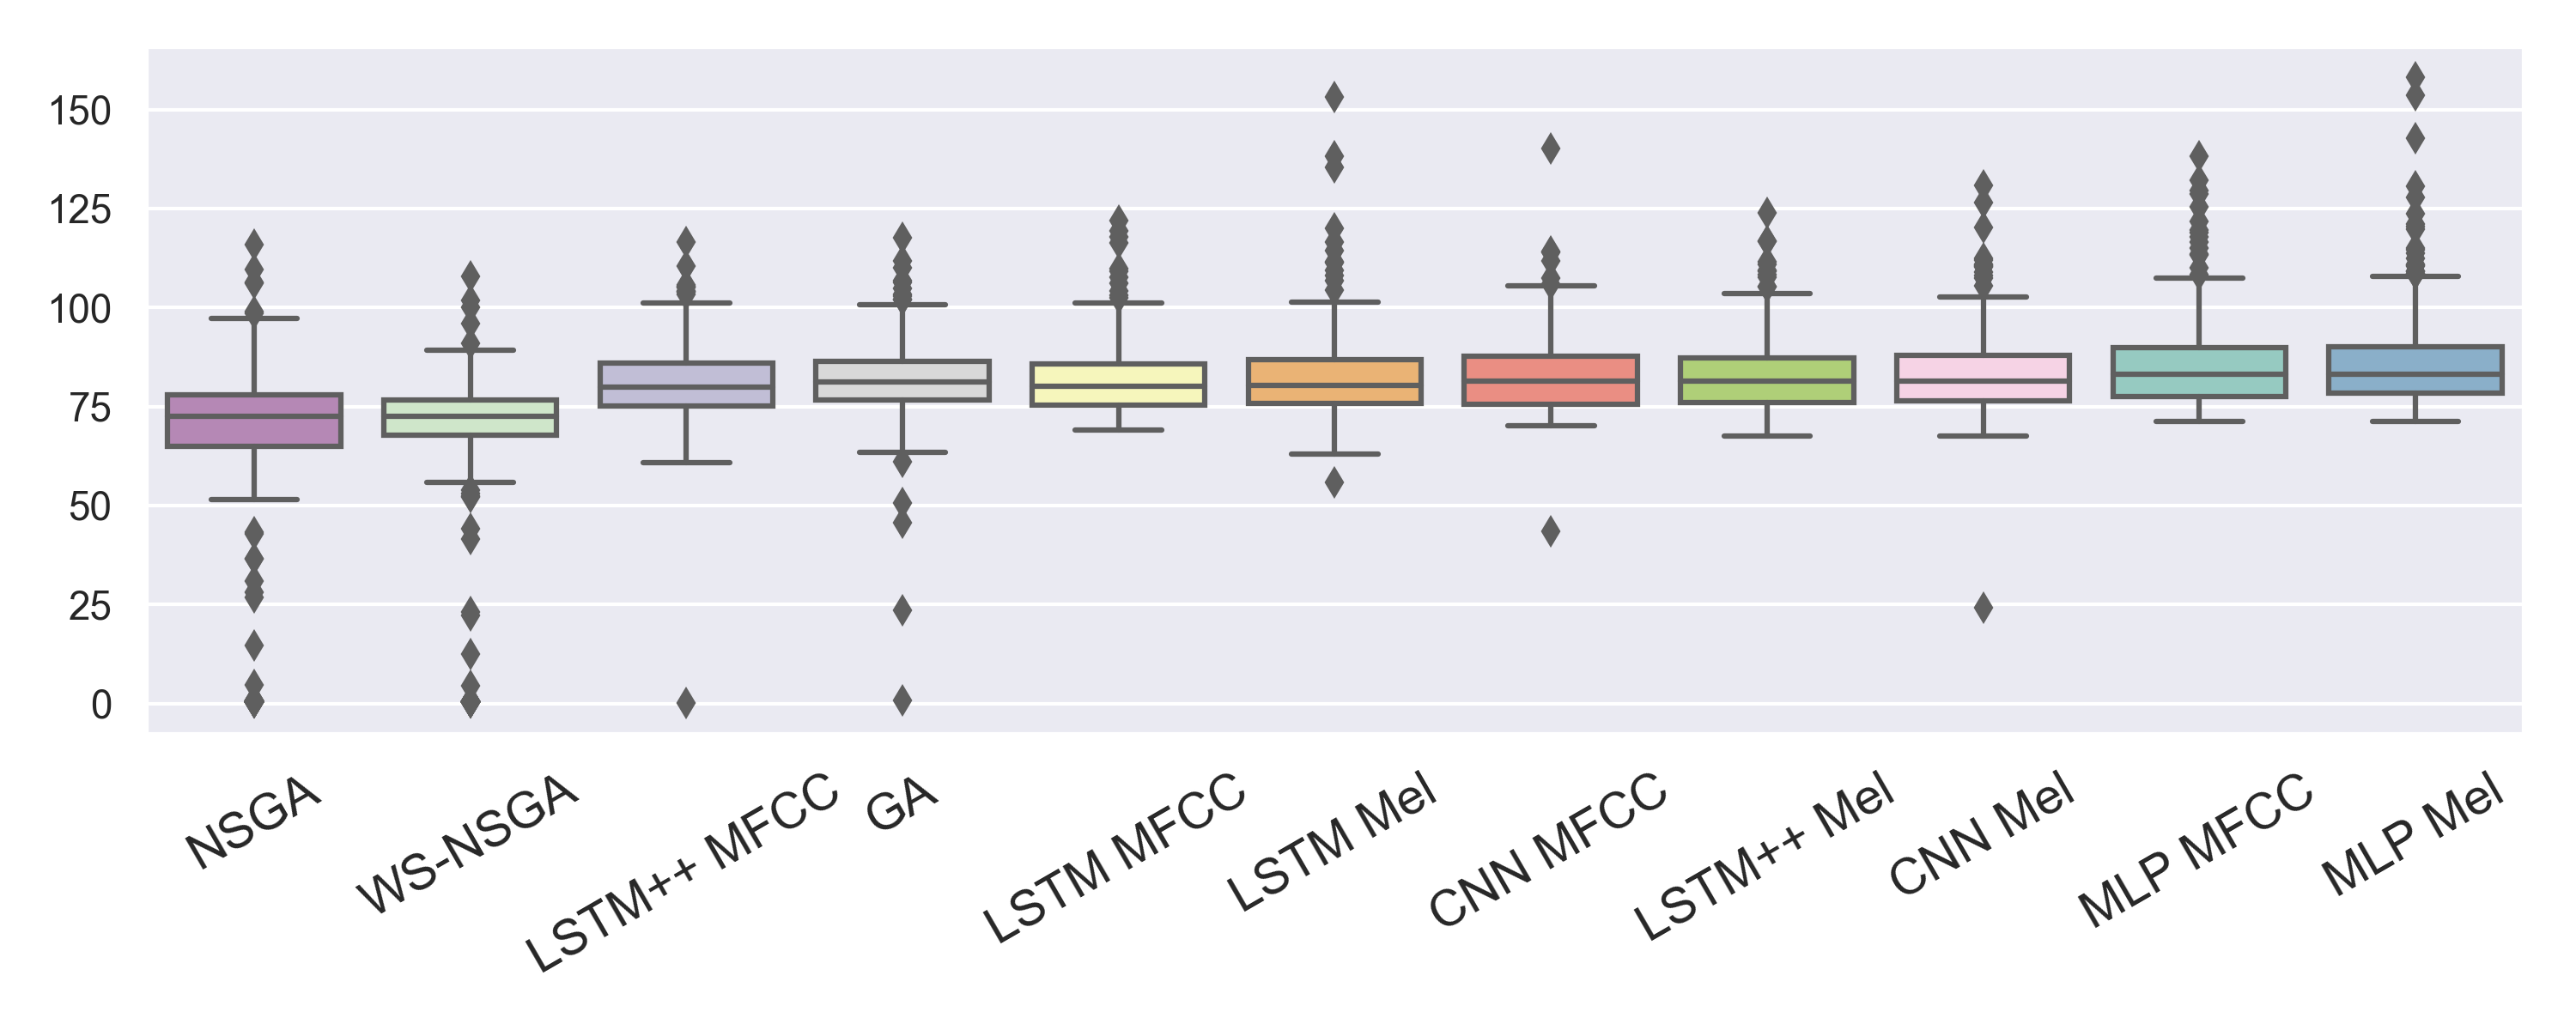
\includegraphics[width=\textwidth]{figures/inverse-synth/lsd_boxplot.png}
        \caption{Log Spectral Distance}
        \label{fig:lsd}
    \end{subfigure}
    \begin{subfigure}[b]{0.99\textwidth}
        \centering
        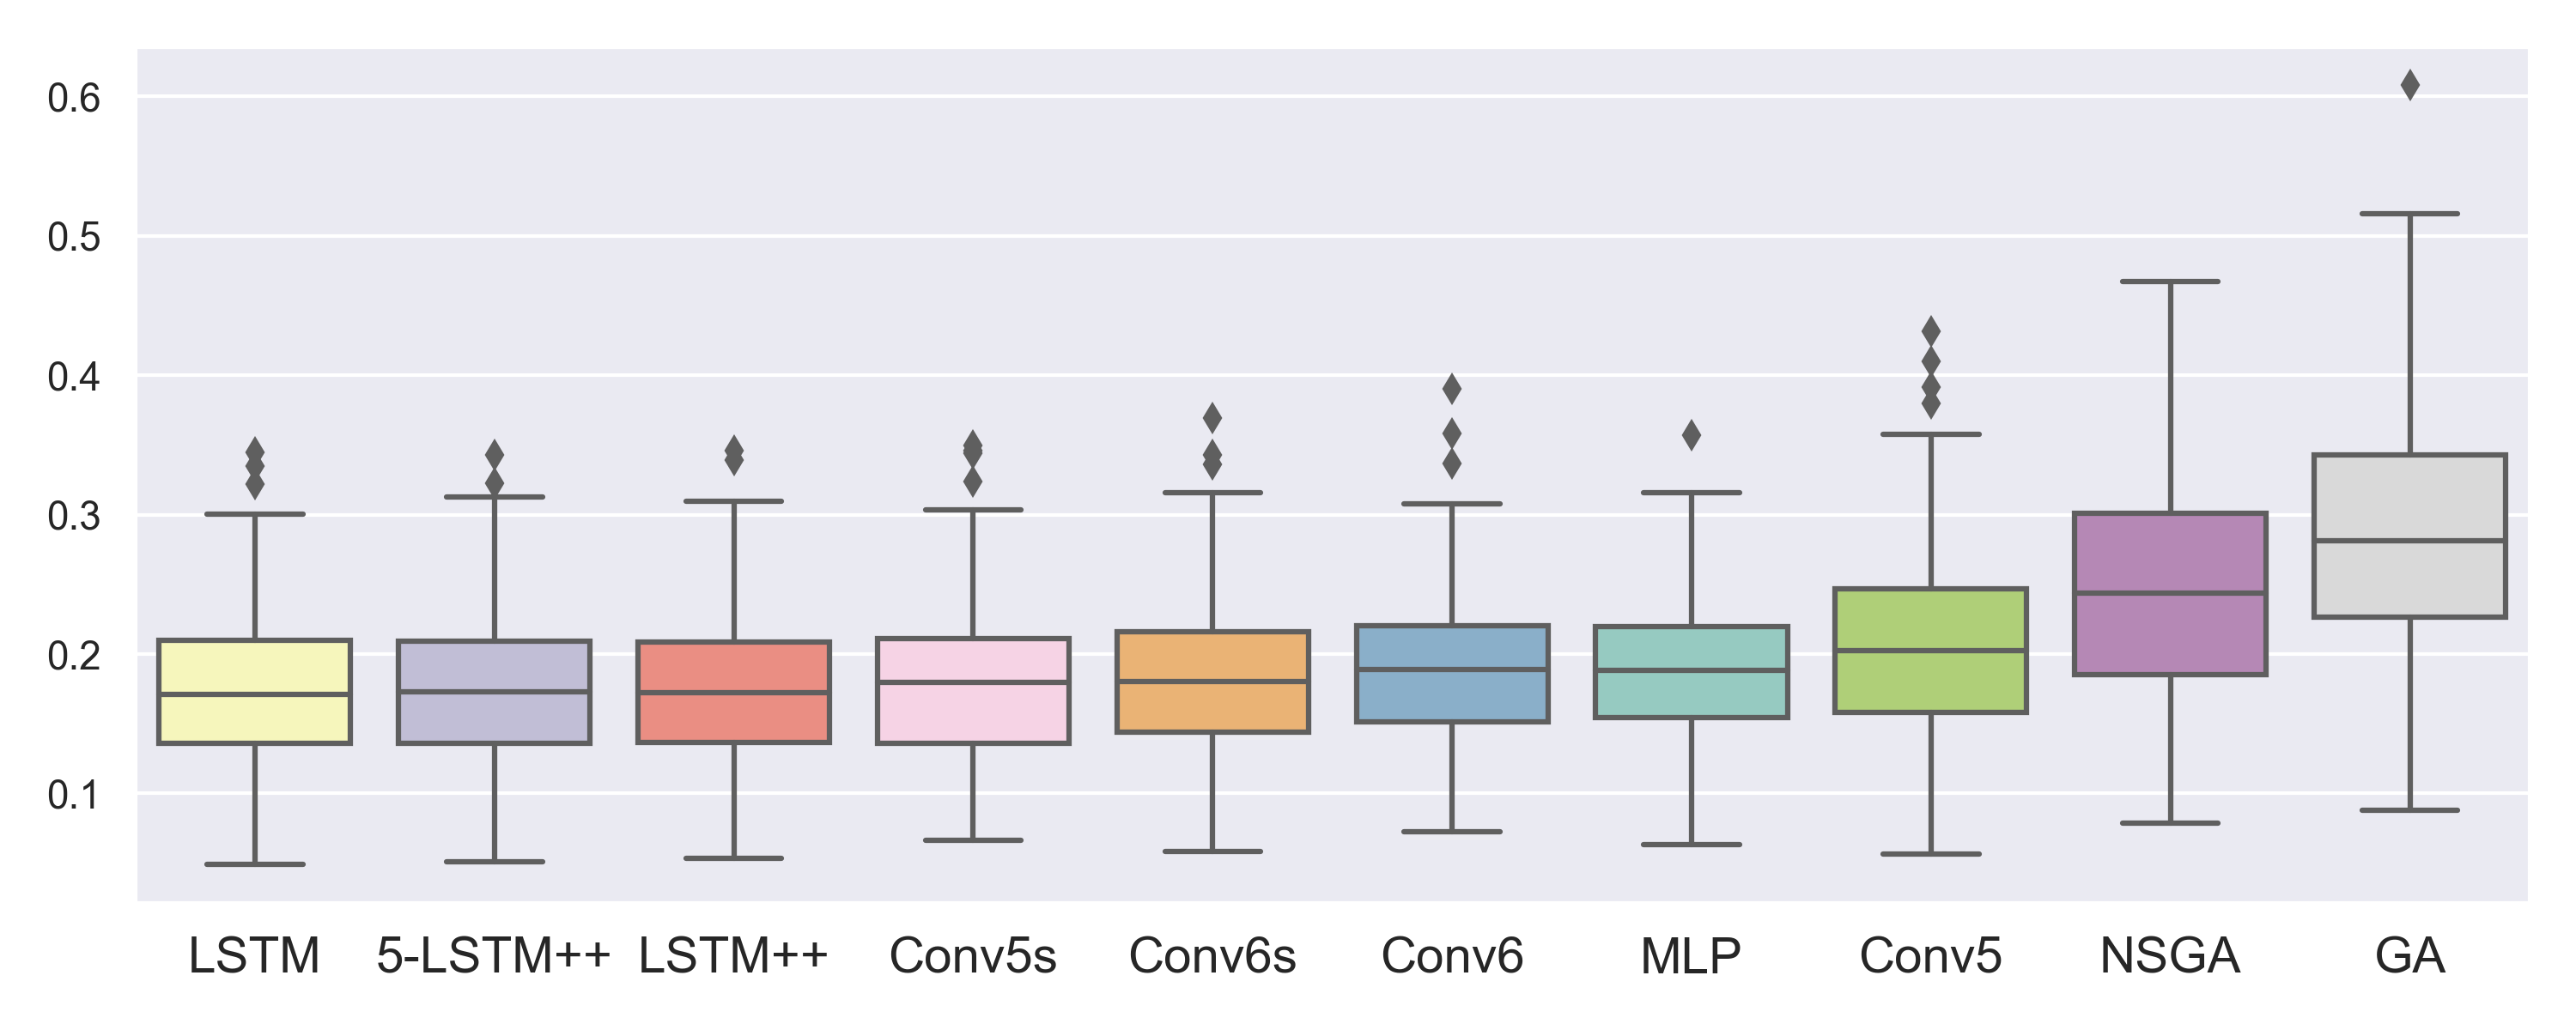
\includegraphics[width=\textwidth]{figures/inverse-synth/parameter_boxplot.png}
        \caption{Parameter MSE}
        \label{fig:param-mse}
    \end{subfigure}
    \caption{Boxplots showing the objective measurements comparing each estimation method using a 250 sample evaluation dataset for sound matching.}
    \label{fig:eval-bocplot}
\end{figure}


% All estimators were run on each one of the 25 target sounds using the \mintinline{python}{SoundMatch} class. This resulted in a set of audio files generated from $Dexed$ using the estimated parameters from each estimator run on each of the 25 target sounds. All of the resulting sounds are available for listening online on the SpiegeLib docs page\footnote{\url{https://spiegelib.github.io/spiegelib/examples/fm_sound_match_pages/fm_sound_match_listen.html}}. Quantitative and qualitative evaluation was conducted on these sounds.

% \subsection{Quantitative Evaluation}
% Evaluation was conducted by comparing the predicted audio files to the target audio using MAE computed on MFCCs, which is the same method that was used during evaluation by Yee-King et al. \cite{yee2018automatic}. Results for mean absolute error (MAE) which have been summarized using mean, standard deviation, minimum, and maximum, are shown for each estimator in table \ref{tbl:sound_match_eval}. Both GAs performed better than the deep learning approaches with the NSGA III having the best overall score. For deep learning approaches, the LSTM++ model achieved the best mean score.

% % TODO informal listening based on MAE so I can comment on the results in terms of MAE

% Histograms of the the MAE were also plotted for each estimator using the \mintinline{python}{plot_hist()} method in \mintinline{python}{EvaluationBase}. Histograms of the MAE for all predictions made by all estimators are shown in figure \ref{fig:group_hist}. These plots clearly show the NSGA III as the winner in terms of MFCC MAE; 24/25 of the predicted sounds have an MAE less than 2.5 (the smallest histogram bin), and the other sound is still less than 5. For the deep learning models, the LSTM++ performed the best overall, however the LSTM model produced more results that had a MAE less than 2.5. The MLP model performed the worst overall and the histogram shows a wide range of results, the MLP also produced a result with the worst individual score of 34.12. The CNN model performed only slightly better than the MLP and had no predictions with a score less than 2.5.

\begin{table}[p]
\centering
\begin{tabular}{r|ccc|ccc|c}
\toprule
{} & \multicolumn{3}{c}{EG Rate} & \multicolumn{3}{c}{EG Level} & {} \\
{} & 2 & 3 & 4 & 2 & 3 & 4 & Mean \\
\midrule
MLP      &     0.0310 &     0.1847 &     0.1988 &      0.1580 &      0.1437 &      0.2379 &   0.1590 \\
LSTM     &     0.0183 &     0.1458 &     0.1923 &      0.1086 &      0.1160 &      0.2429 &   0.1373 \\
5-LSTM++ &     0.0216 &     0.1464 &     0.1782 &      0.0979 &      0.1134 &      0.2395 &   0.1328 \\
LSTM++   &     0.0223 &     0.1555 &     0.1788 &      0.1217 &      0.1057 &      0.2245 &   0.1348 \\
Conv6    &     0.0325 &     0.1837 &     0.1773 &      0.1167 &      0.1421 &      0.2296 &   0.1470 \\
Conv6s   &     0.0291 &     0.1587 &     0.1588 &      0.1303 &      0.1094 &      0.2308 &   0.1362 \\
Conv5    &     0.0494 &     0.2176 &     0.1973 &      0.1467 &      0.1330 &      0.2384 &   0.1637 \\
Conv5s   &     0.0255 &     0.1618 &     0.1515 &      0.1181 &      0.1076 &      0.2357 &   0.1334 \\
GA       &     0.0330 &     0.2983 &     0.2712 &      0.2254 &      0.2173 &      0.3321 &   0.2295 \\
NSGA     &     0.0097 &     0.2515 &     0.2853 &      0.1839 &      0.1839 &      0.3048 &   0.2032 \\
\midrule
Mean  &     0.0272 &     0.1904 &     0.1990 &      0.1407 &      0.1372 &      0.2516 &   0.1577 \\
\bottomrule
\end{tabular}
\caption{Results from sound matching evaluation}
\label{tbl:param_eval_eg}
\end{table}

\begin{table}[p]
\centering
\begin{tabular}{r|ccc|c}
\toprule
{} & \multicolumn{3}{c}{Oscillator Frequency} & {} \\
{} & Coarse & Fine & Detune & Mean \\
\midrule
MLP      &    0.0678 &  0.2390 &      0.2576 & 0.1881 \\
LSTM     &    0.0718 &  0.2368 &      0.2573 & 0.1886 \\
5-LSTM++ &    0.0723 &  0.2464 &      0.2563 & 0.1917 \\
LSTM++   &    0.0707 &  0.2328 &      0.2612 & 0.1882 \\
Conv6    &    0.0779 &  0.2364 &      0.2592 & 0.1912 \\
Conv6s   &    0.0773 &  0.2533 &      0.2529 & 0.1945 \\
Conv5    &    0.0815 &  0.2379 &      0.2555 & 0.1917 \\
Conv5s   &    0.0704 &  0.2400 &      0.2622 & 0.1909 \\
GA       &    0.0911 &  0.2793 &      0.3656 & 0.2454 \\
NSGA     &    0.0728 &  0.2344 &      0.2555 & 0.1876 \\
\midrule
Mean     &    0.0754 &  0.2436 &      0.2683 & 0.1958 \\
\bottomrule
\end{tabular}
\caption{Results from sound matching evaluation}
\label{tbl:param_eval_osc}
\end{table}

% Maybe add some spectrograms?
% \subsection{Qualitative Evaluation}
% Spectrograms of one target sound and predictions made by each of the estimators for that target are shown in figure \ref{fig:group_spect}. The selected example was one of the most challenging targets; both the GAs, the LSTM, and the MLP received their worst individual score on it. The most clear difference between the spectrograms can be seen in the temporal evaluation of the harmonics, which is caused by the EG applied to the amplitude of the second operator. In the target the envelope has two obvious components: 1) gradually descending over the first half, and then 2) remaining constant for the remainder of the sound. All the predictions have a similar shape, however only the NSGA III is able to match the shape of of those two sections of the envelope. The MLP, which performed the worst, has two envelope sections, but the first section descends too radpidly and then the constant section is at the incorrect amplitude.

% Another aspect of the spectrograms that can be identified are periodic amplitude modulations occuring along the horizontal axis of the harmonics. These show up as period dark notches on the harmonic. These spacing between the horizontal notches indicates the tuning of the second operator that is modulating the frequency of the first operator. In the target this modulation pattern shows up in the first half of the clip, but not the second. Only the NSGA III was able to correctly match the tuning in both sections of the audio. 

% Did I mess up the charts for the CNN and the GA?? Those shouldn't be different I don't think?

% \begin{figure}[t]
% \begin{center}
% 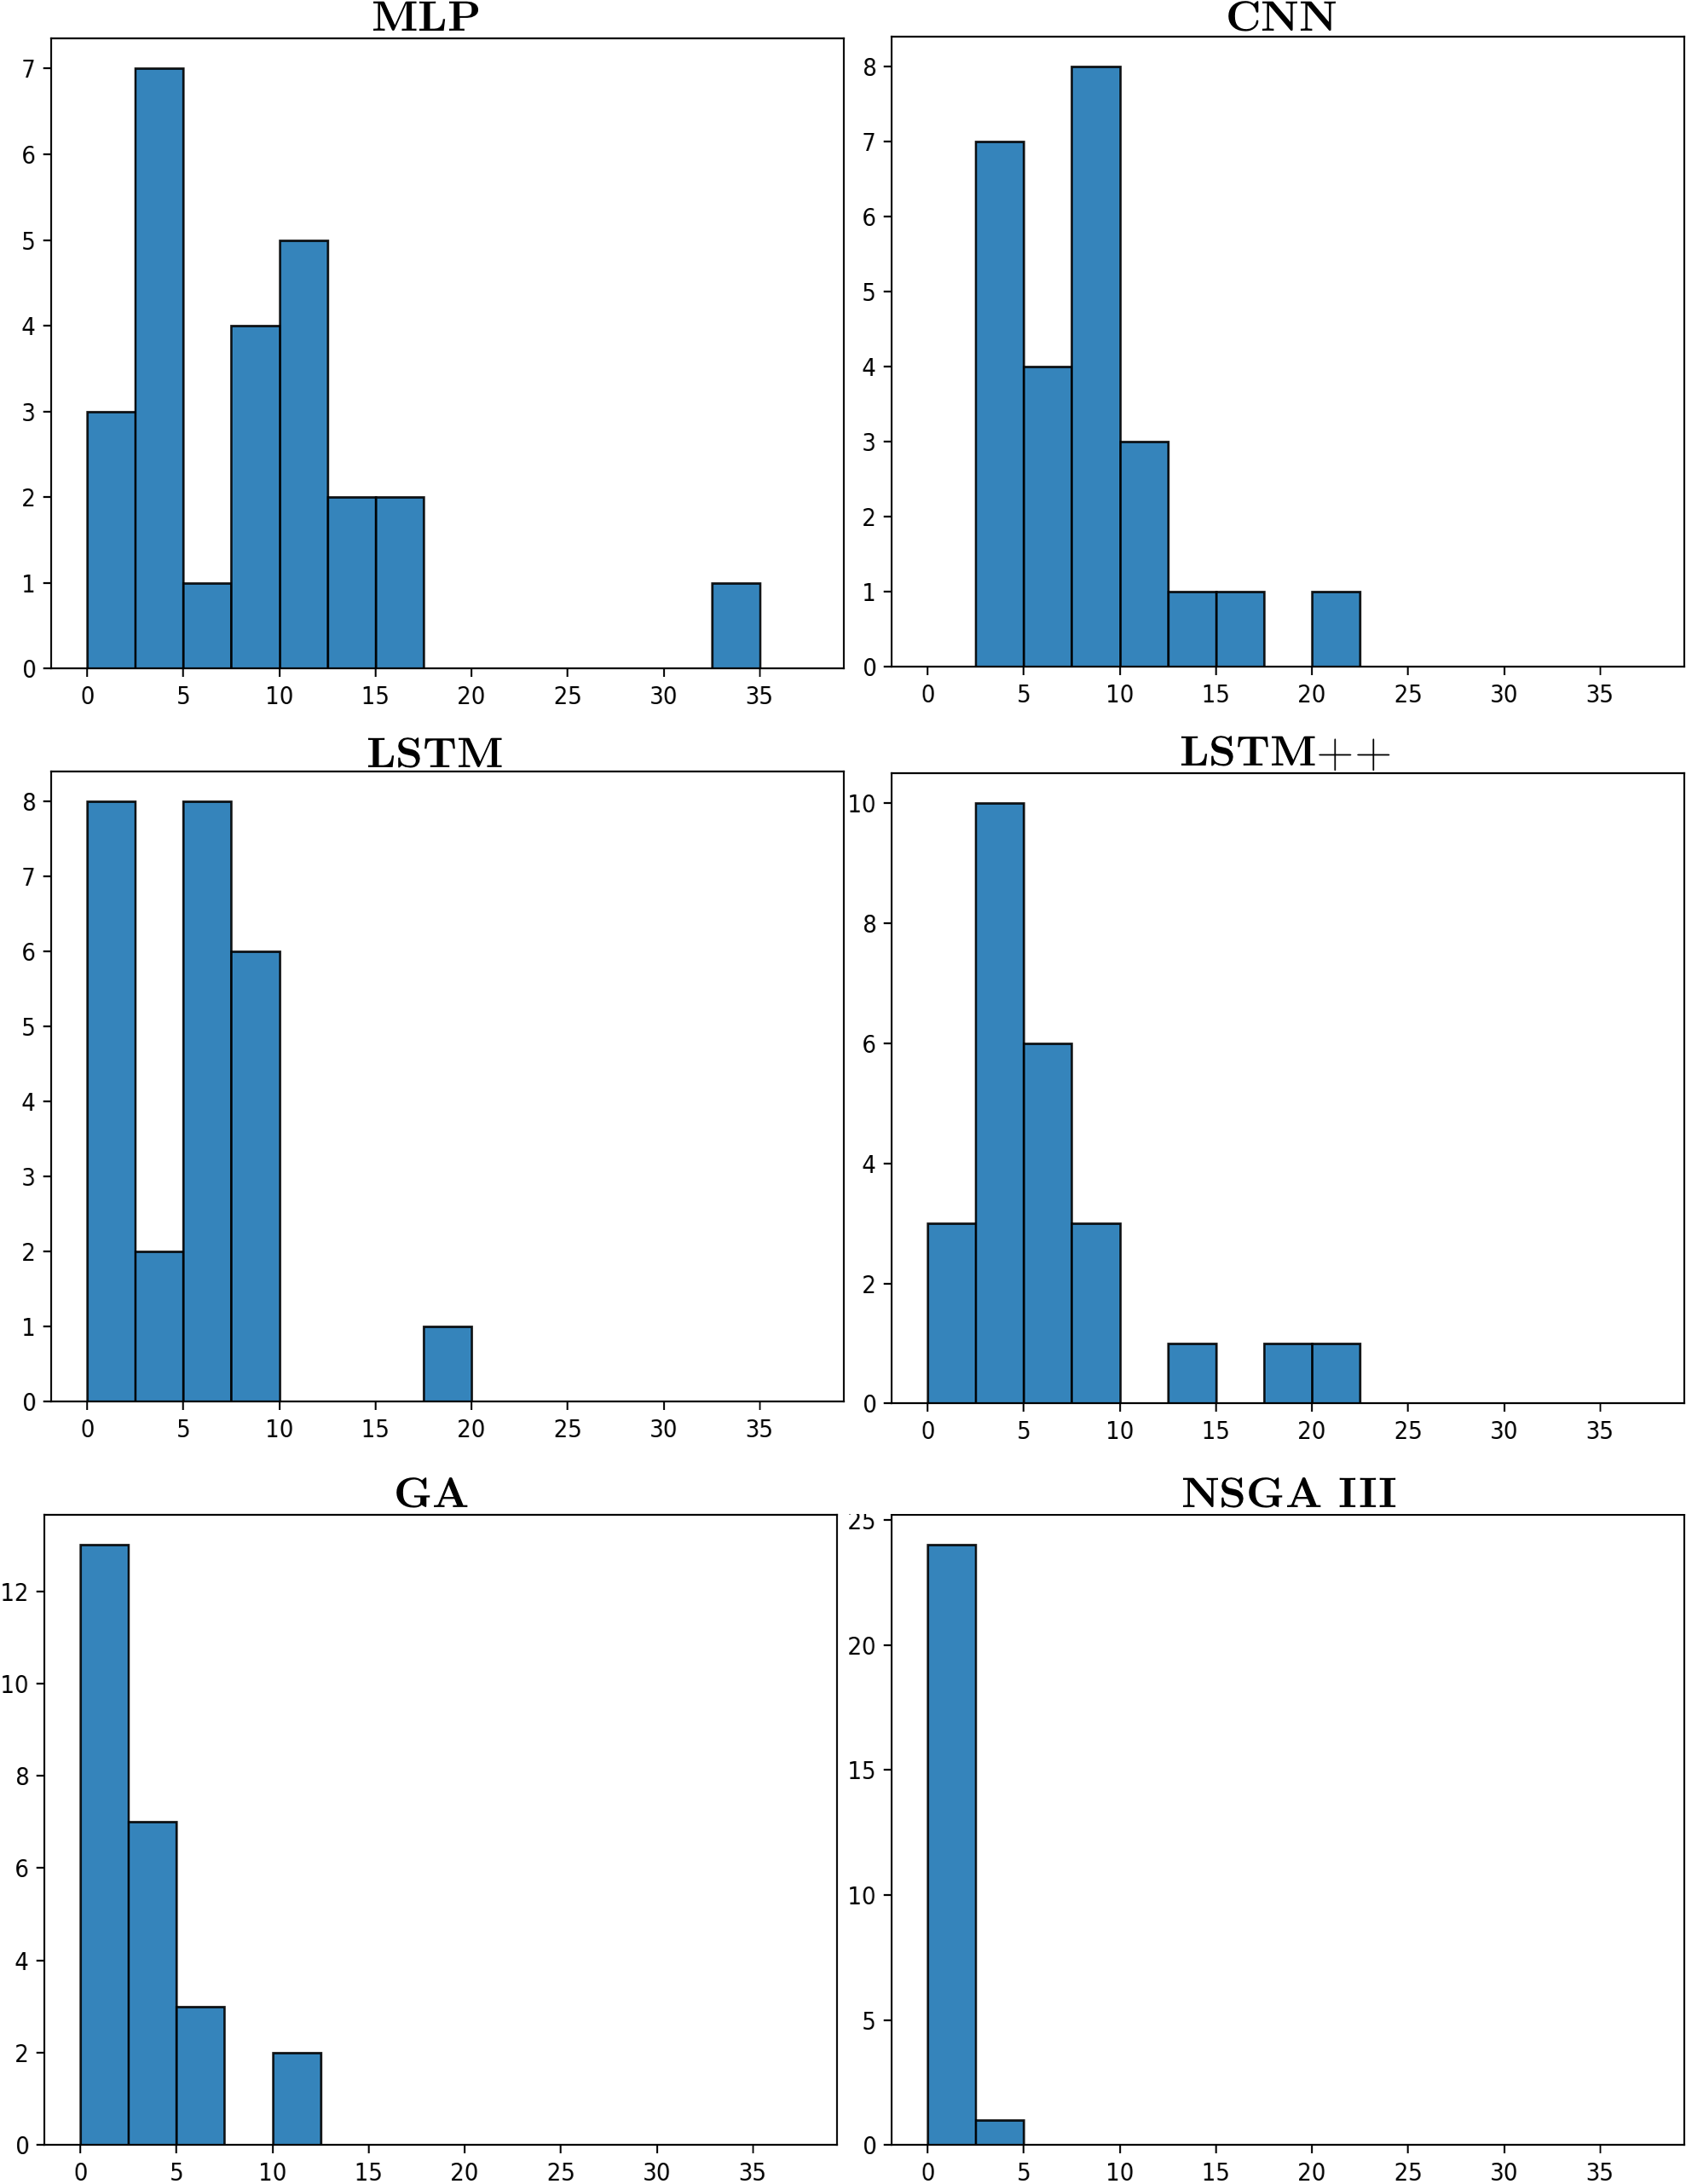
\includegraphics[width=0.75\textwidth]{hist_group_v3.png}
% \caption{Histogram shows the MAE values resulting from MFCC evaluation run on a set of 25 sound targets for all estimators. Lower MAE values indicate a closer sound match.}
% \label{fig:group_hist}
% \end{center}
% \end{figure}

% \begin{figure}[t]
% \begin{center}
% 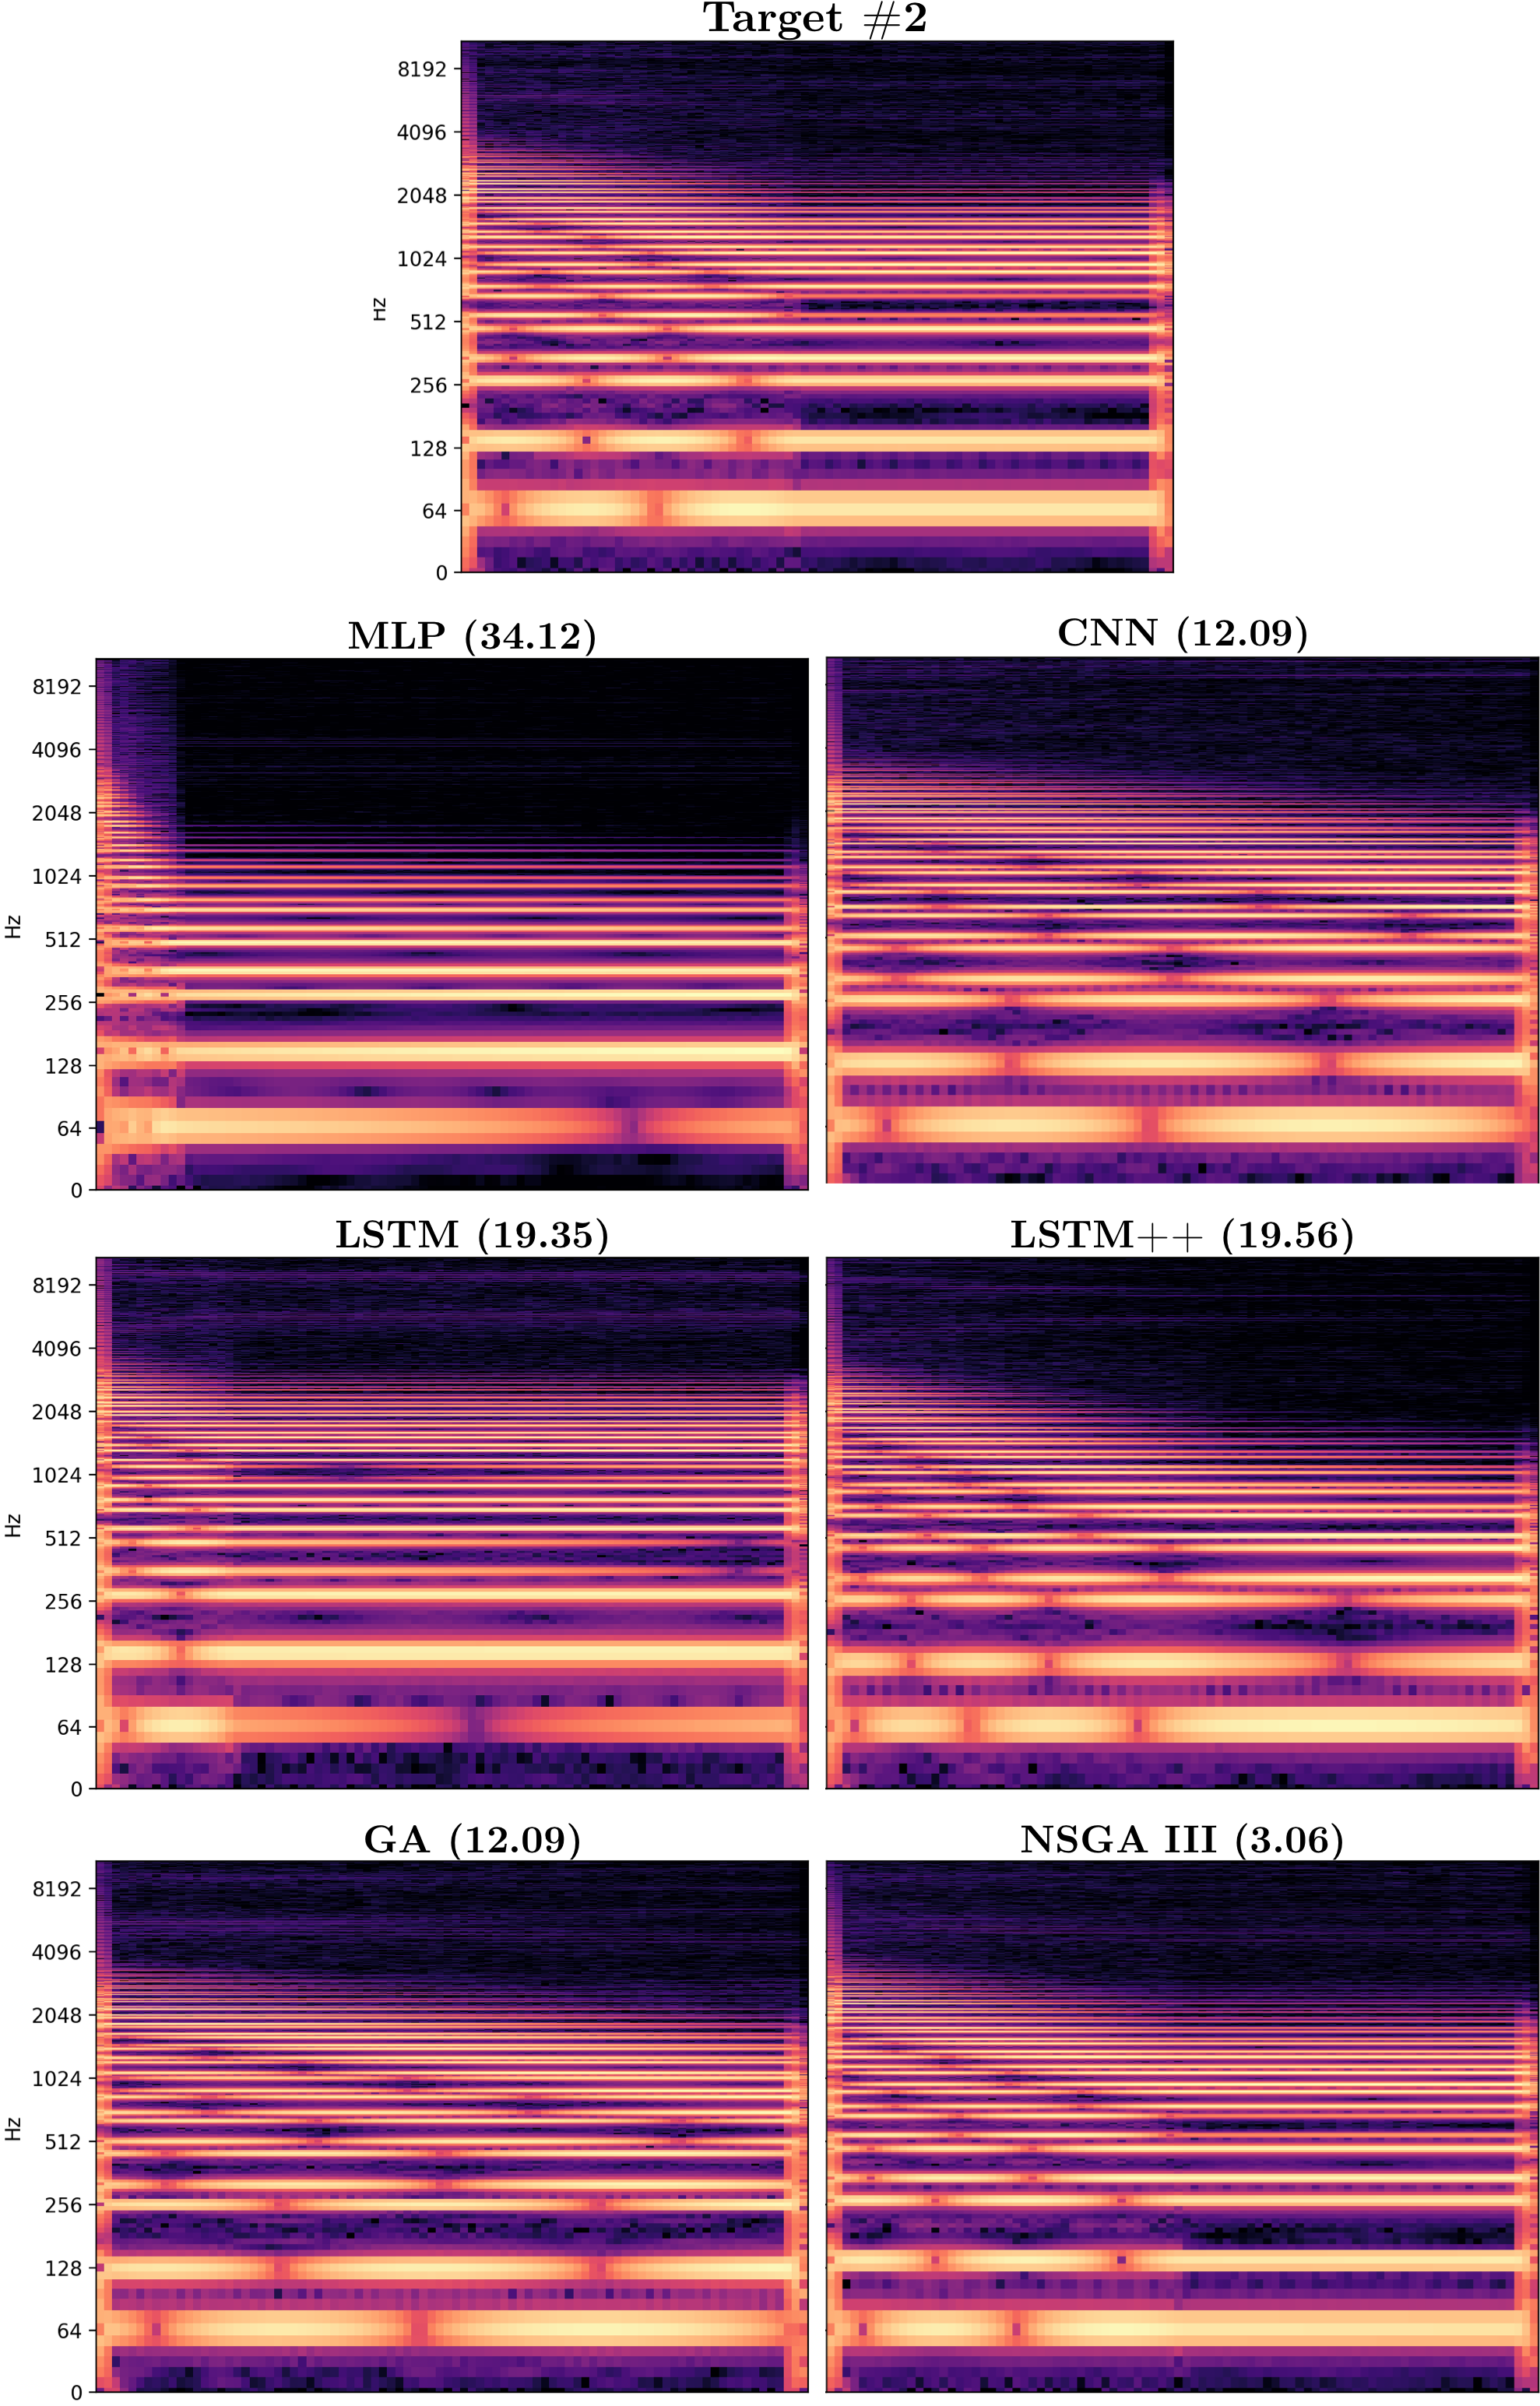
\includegraphics[width=0.75\textwidth]{spect_group_v1.png}
% \caption{Spectrogram plots of a target sound and sound match predictions made by each estimator. The value next to the estimator name is the MAE value from MFCC evaluation for that prediction (lower MAE values indicate a closer match).}
% \label{fig:group_spect}
% \end{center}
% \end{figure}

% I think this can be removed?
% To evaluate to the resulting predictions the \mintinline{python}{MFCCEval} class was used, which calculates error and distance metrics on MFCCs of a target and prediction. Results for mean absolute error (MAE) which have been summarized using mean, standard deviation, minimum, and maximum, are shown for each estimator in table \ref{tbl:sound_match_eval}. Both GAs performed better than the deep learning approaches with the NSGA III having the best overall score. For deep learning approaches, the LSTM++ model achieved the best mean score. Histograms of the the MAE were also plotted for each estimator using the \mintinline{python}{plot_hist()} method in \mintinline{python}{EvaluationBase}. Histograms of the MAE for all predictions made by all estimators are shown in figure \ref{fig:group_hist}. Spectrograms of one target sound and sound match predictions made by each of the estimators for that target are shown in figure \ref{fig:group_spect}. For this particular target, spectrograms reveal that while the frequency and distribution of the harmonics was relatively close for each estimation, all estimators except for the NSGA III struggled with matching the temporal envelope of the spectrum.

\section{Discussion}
\label{sec:inverse-synth-discuss}

 These results shed light an important aspect of synthesizer programming: high parameter error does not necessarily equate to high auditory error. The NSGA-III algorithm consistently outperformed all of the other techniques in both the audio evaluation metrics, despite being outperformed by all the deep learning models in terms of parameter error. 

% This is one of the benefits of the GAs over the deep learning approaches, the error between the target and the prediction can be measured directly on the audio, as opposed to measuring the error based on the parameter settings. The downside of this is that GAs are mu

\section{Conclusion}

- Conducted an inverse synthesis experiment on a VST software synthesizer Dexed
- Results showed that the GAs performed the best via objective evaluation
- LSTM++ model performed the best out of the deep learning models
- Comparison of the search versus modelling methods for inverse synthesis
- Discussion of the parameter sampling methods -- uniform sampling may not provide the best method for training the deep learning models to learn sounds that a human might program
- Challenges associated with programming a VST software synth




%\section{Related Work}
%- Go over the three specific papers that SpiegeLib and the experiments are based on.
%- Deep learning: Fully connected and recursive nets: \cite{yee2018automatic}, Convolutional Nets: \cite{barkan2019inversynth}, Genetic Algorithms: \cite{tatar2016automatic}
%
%\subsection{Recurrent Neural Networks}
%One of the first works on the application of deep learning to the inverse synthesis problem was published by Matthew Yee-King et al. \cite{yee2018automatic} in 2018. The main contribution of their work was an experiment that showed the effectiveness of a type of recurrent neural networks (RNN) called long short-term memory (LSTM) networks at sound matching on an FM synthesizer audio plugin. RNNs were developed to handle time-series data and receive ordered data which is successively fed into the network architecture. As data is fed into the networks, activation states are stored internally and help to provide temporal context in latter stages of computation. RNNs have been particularly successful for audio generation problems \cite{oord2016wavenet, engel2017neural}. 
%
%Yee-King er al. also experimented with additional machine learning techniques including genetic algorithm (GA), Hill-climber, and  multi-layer perceptron (MLP) methods. They also compared two RNN models: a regular LSTM network as well as a modified LSTM network that had a bi-directional LSTM layer as well as several highway layers, they called this network an LSTM++. Their methodology compared a set of algorithms on a series of successfully more challenging problems on the open-source FM synthesizer Dexed\footnote{\url{https://asb2m10.github.io/dexed/}}. Each problem was focused on programming a subset of the parameters in Dexed; a larger subset was used for each successive problem. A dataset of audio samples paired with the parameters used to generate the audio was created for training each of the deep learning models. Mel-frequency Cepstral Coefficients (MFCCs) were used as input for each of the models. The results were evaluated by looking at the error between MFCCs from target sound and a predicted sound. Results showed that the hill-climber algorithm and the LSTM++ model performed the best. The LSTM++ model showed significant improvements over the other deep learning methods, however the hill-climber performed the best on a majority of the tasks.
%
%Their methodology and software provided a basis for the work presented in the chapter and in the development of SpiegeLib.
%
%\subsection{Convolutional Neural Networks}
%Barkan et al. explored convolutional neural networks (CNNs) applied to the inverse synthesis problem in their work which presenting InverSynth \cite{barkan2019deep}. The CNN has been used extensively for image related deep learning tasks and has recently been used successfully in music and audio related tasks including music genre classification \cite{choi2016automatic} and neural audio generation \cite{donahue2018adversarial}. A key feature of CNNs is the use of shared filters that perform convolutions and produce representations at various levels of specificity. The shared filters has allowed them to process large input data such as images and audio with relatively few parameters compared to their fully connected counterparts. 
%
%In their work, Barkan et al. experiment with several different CNN architectures and compare them to a few different fully-connected networks. The focus of their research is performing inverse synthesis on a custom built four oscillator FM synthesizer. They frame the inverse synthesis problem as a classification problem and quantize each of the 23 continuous synthesizer parameters into 16 discrete states. As input they experiment with both STFT as well as raw time-domain audio. Because of the size of these input they created different input representations for the fully-connected networks, for these they used a selection of hand-picked audio features defined in work by Itoyama et al. \cite{itoyama2014parameter}.
%
%Results were evaluated using four different objective methods which evaluate both the ability of the model to match the parameters as well as to reconstruct the target audio. The evaluation metrics used are:
%1) Mean Percentile Rank (MPR): ranked position of the correct class measured against predicted classes in the output. Computed independently on each of the 23 synthesizer parameters, each parameter has 16 classes.
%2) Top-k Mean Accuracy: measures whether the correct class is among the top-k predicted classes for each parameter.
%3) Mean Absolute Error (MAE): this measures the error of the predicted class for each parameter.
%4) Spectral Reconstruction Quality: predicted parameters are used to synthesize a predicted audio. The predicted audio is compared against the target audio using error metrics calculated on the STFT and FT representations.
%
%They also conducted a subjective listening experiment which measured the quality of the target audio to the predicted audio for a selection of the methods. Results from the objective and subjective evaluation showed that the depth of the convolutional network played an important role in the quality of the estimator and the best performing networks were two different networks with 6-layers.


% \begin{table}[t]
% \centering
% \caption{Results from sound matching evaluation}
% \label{tbl:sound_match_eval}
% \begin{threeparttable}
% \begin{tabular}{l|cccc}
% \toprule
% $Method$ & $Mean$ & $SD$ & $Min$ & $Max$ \\
% \midrule
% $MLP$ & 8.55 & 6.77 & 1.92 & 34.12 \\
% $CNN$ & 7.88 & 4.26 & 2.68 & 20.89 \\
% $LSTM$ & 6.12 & 3.76 & 1.20 & 19.36 \\
% $LSTM++$ & 4.91 & 6.50 & 2.12 & 21.51 \\
% $GA$ & 2.25 & 2.58 & 0.70 & 11.17 \\
% $NSGA III$ & \textbf{0.81} & \textbf{0.89} & \textbf{0.001} & \textbf{3.06} \\
% \bottomrule
% \end{tabular}
% \begin{tablenotes}[para, flushleft]
% \footnotesize
% \item Values shown are calculated from the mean absolute error (MAE) calculated during MFCC evaluation. Smaller MAE values indicate more similar matches. The NSGA III estimator received the best scores, which are shown in bold font.
% \end{tablenotes}
% \end{threeparttable}
% %\vspace{5mm}
% \end{table}